% Основной файл ВКР (рекомендуемый старт)
% Сборка: latexmk -pdf main.tex
\documentclass[a4paper,14pt]{extarticle}

% Шаблон оформления (поля/интервал/заголовки)
\usepackage{spbudiploma_tempora}

% Часто используемые пакеты (минимальный набор)
\usepackage{amsmath,amssymb}
\usepackage[pdftex]{graphicx}
\usepackage{csquotes}
\usepackage{longtable}
\usepackage{placeins}
\usepackage{tikz}
\usepackage{float}
\usepackage[ruled,vlined]{algorithm2e}
\usepackage{caption}
\usepackage{url}
\urlstyle{same}
\usetikzlibrary{arrows.meta,positioning,fit,calc,matrix}
\usetikzlibrary{matrix}

% Библиография по ГОСТ (biblatex + biber)
% Основной вариант: biblatex-gost (style=gost-numeric).
% Если biblatex-gost не установлен, используем fallback style=numeric.
\IfFileExists{gost-numeric.bbx}{
  \usepackage[
    backend=biber,
    style=gost-numeric,
    hyperref=true,
    language=auto,
    autolang=other,
    sorting=none
  ]{biblatex}
}{
  \usepackage[
    backend=biber,
    style=numeric,
    hyperref=true,
    sorting=none
  ]{biblatex}
  \typeout{WARNING: biblatex-gost not found; using style=numeric. Install biblatex-gost for GOST formatting.}
}
\addbibresource{references.bib}

% Черновик структуры ВКР:
%
% Введение
% - актуальность распределённого отказоустойчивого хранения;
% - проблема выбора между репликацией и erasure coding;
% - идея адаптивного изменения схемы хранения;
% - цель работы;
% - задачи работы;
% - ограничения постановки: append-only, background recoding, без фонового repair
%   в базовой версии.
%
% Обзор литературы
% - репликация в распределённых системах хранения;
% - erasure coding и коды Рида--Соломона;
% - LRC и локальное восстановление;
% - convertible codes;
% - LRCC как расширение convertible codes на LRC;
% - Morph и lifecycle-aware storage;
% - выводы по обзору литературы.
%
% Глава 1. Теоретические основы адаптивного кодирования данных
% 1.1 Модель распределённого хранения и отказов
%     - объекты, фрагменты, узлы и домены отказа;
%     - append-only постановка и чтение уже записанных данных.
% 1.2 Репликация и глобальная избыточность
%     - репликация как частный случай избыточности;
%     - коды Рида--Соломона и global parity.
% 1.3 Локально восстанавливаемые коды
%     - local parity, local group и local repair;
%     - зачем локальность нужна при одиночных отказах.
% 1.4 Конвертируемые коды и LRCC
%     - переходы между схемами и стоимость конверсии;
%     - LRCC как locally repairable convertible codes: LRC на базе модели
%       конверсии, а не просто ещё один вариант LRC;
%     - Morph упоминается внутри этого подраздела как практическое применение
%       LRCC/convertible codes, а не как источник новой теории LRCC.
% 1.5 Гибридная схема Hy(r, LRCC(d,l,g))
%     - единое состояние для реплик, local parity и global parity;
%     - условие устойчивости к трём отказам.
% 1.6 Чтение при отказах и ожидаемая стоимость чтения
%     - normal read, degraded read и background repair;
%     - E[io] через вероятности числа отказов.
% 1.7 Температура данных и функция полезности перехода
%     - EWMA-модель температуры;
%     - pressure по месту и expected read IO;
%     - score transition как уменьшение pressure на единицу работы.
%
% Глава 2. Архитектура предлагаемого решения
% - общая схема системы;
% - модель объекта, stripe, scheme и chunk;
% - placement policy и anti-affinity;
% - локализация parity и placement slots;
% - recoder и допустимые переходы между схемами;
% - degraded read path;
% - локальные планировщики;
% - глобальный планировщик;
% - функция полезности перехода;
% - обработка конфликтов и ограничение фоновых переходов.
%
% Глава 3. Реализация системы
% - хранилище метаданных объектов и схем;
% - представление физических чанков и ссылок на них;
% - реализация LRCC parity;
% - реализация RS/Vandermonde global parity над GF(2^8);
% - реализация degraded read для 1--3 отказов;
% - реализация переходов replica <-> parity;
% - реализация temperature pipeline;
% - реализация local/global planner loop;
% - механизм фоновых delayed transitions;
% - набор поддерживаемых сценариев работы.
%
% Глава 4. Анализ экспериментов
% - цель и постановка экспериментов;
% - метрики и baseline-сценарии;
% - холодные данные;
% - длительная запись и фоновые переходы;
% - неравномерная температура данных;
% - чтения при отказах;
% - смешанный жизненный цикл;
% - выводы по экспериментам.
%
% Глава 5. Ограничения и направления дальнейшего развития
% - ограничения текущей реализации;
% - background repair engine;
% - merge/split схем;
% - более точная модель latency, bandwidth и fanout;
% - масштабирование planner ownership;
% - проверка на реальных production traces;
% - возможность интеграции с существующими storage systems.
%
% Заключение
% - выполненные результаты;
% - соответствие цели и задачам;
% - основные выводы;
% - что выносится на защиту.

\begin{document}

% 1) Титульный лист
% Титульный лист ВКР СПбГУ.

% Временное удаление колонтитулов на титульном листе
\newgeometry{left=30mm, top=20mm, right=15mm, bottom=20mm, nohead, nofoot}
\begin{titlepage}
\begin{center}

\textbf{Санкт--Петербургский государственный университет}

\vspace{35mm}

\textbf{\textit{\large ДОБРЕНКОВА Лия Сергеевна}} \\[8mm]
\textbf{\large Выпускная квалификационная работа}\\[3mm]
\begin{minipage}{0.9\textwidth}
\centering
\textbf{\textit{\large Разработка гибридной системы erasure coding и репликации на основе температуры данных}}
\end{minipage}

\vspace{20mm}
Уровень образования: бакалавриат\\
Направление 02.03.02 «Фундаментальная информатика и информационные технологии»\\
Основная образовательная программа СВ.5190.2022\\
«Большие данные и распределенная цифровая платформа»\\[25mm]

\begin{flushright}
\begin{minipage}[t]{0.70\textwidth}
{Научный руководитель:}\\
профессор, заведующий кафедрой фундаментальной\\
информатики и распределенных систем,\\
д.ф.-м.н. Утешев Алексей Юрьевич

\vspace{10mm}

{Рецензент:}\\
старший преподаватель, кафедра фундаментальной\\
информатики и распределенных систем,\\
Давыденко Александр Александрович
\end{minipage}
\end{flushright}

\vfill

{Санкт-Петербург}\\
\par{2026 г.}
\end{center}
\end{titlepage}

% Возвращаем настройки geometry обратно (то, что объявлено в преамбуле)
\restoregeometry
% Исключаем титульный лист из нумерации страниц
\addtocounter{page}{1}



% 2) Оглавление
\tableofcontents
\pagebreak

% 3) Основной текст
\specialsection{Введение}

В настоящее время количество доступной информации постоянно увеличивается.
Современные распределённые системы хранения должны одновременно обеспечивать
высокую доступность данных, устойчивость к отказам оборудования и эффективное
использование дискового пространства. Эти требования особенно важны для
крупных хранилищ, где данные размещаются на множестве серверов, а отказы
отдельных дисков или узлов являются не исключением, а штатной частью
эксплуатации \cite{shen2024erasurecoding}. В таких условиях способ
организации избыточности напрямую влияет на стоимость хранения, задержку
чтения и цену восстановления после отказов.

На практике широко используются два основных подхода к отказоустойчивому
хранению: репликация и коды, исправляющие стирания. Репликация проста в
реализации и обеспечивает дешёвое чтение при отказах, но требует большого
расхода дискового пространства. Коды с исправлением стираний, напротив,
позволяют существенно снизить объём избыточных данных, но делают чтение и
восстановление при отказах более дорогими
\cite{huang2012azure,muralidhar2014f4}.

На практике данные нередко сначала хранятся с репликацией, а затем переводятся
в схемы с кодами стираний для снижения расхода места
\cite{li2017ear,kim2024morph}. Однако такой переход сам по себе может быть
дорогим: в распространённой реализации перекодирование сводится к чтению
данных, записи нового представления и удалению старого \cite{kim2024morph}.
Сложность выбора усиливается тем, что нагрузка на данные обычно неравномерна:
разные объекты и участки объектов имеют разную интенсивность чтения, которая
изменяется со временем \cite{levandoski2013hotcold,muralidhar2014f4}.

В работах о хранилищах такую активность часто описывают через температуру
данных: горячие данные получают много запросов, а более холодные данные
читаются реже \cite{muralidhar2014f4,song2024hsm}. В данной работе температура
используется как численная метрика текущей интенсивности чтений, а не только
как принадлежность объекта к одному из заранее заданных классов. При высокой
активности важнее низкая ожидаемая стоимость чтения, при низкой ---
компактность хранения. Кроме того, меняется состояние самого кластера: при
достаточном свободном месте система может предпочитать более быстрые схемы, а
при росте заполненности дисков --- более компактные. Следовательно,
фиксированная схема избыточности может быть либо слишком дорогой по месту, либо
слишком дорогой по чтению, восстановлению и последующему перекодированию.

Таким образом, актуальной становится задача не только выбора одной схемы
избыточности при записи данных, но и управления схемой хранения в течение
жизненного цикла данных. Такая задача требует одновременно учитывать текущую
активность чтений, доступное дисковое пространство и стоимость фоновых
переходов, поскольку само перекодирование может конкурировать с
пользовательской нагрузкой за дисковые и сетевые ресурсы.

В данной работе рассматривается подход, в котором схема хранения является
изменяемым состоянием жизненного цикла данных. Основная идея состоит в том,
чтобы описывать разные формы избыточности в едином пространстве состояний и
выбирать фоновые переходы между ними по функции полезности. В отличие от
фиксированной цепочки переходов, планировщик учитывает текущую температуру
данных, занятое место, ожидаемую стоимость чтения и стоимость фоновой работы.
Формальная модель такого пространства состояний вводится в первой главе.

Работа ориентирована на append-нагрузку: запись новых объектов и дозапись
существующих без изменения уже закрытых полос данных.

Цель работы --- разработать модель и архитектурный подход адаптивного
отказоустойчивого хранения данных с дозаписью, в котором система может
автоматически менять форму избыточности между состояниями с преобладанием
реплик и состояниями с преобладанием проверочных блоков в зависимости от
активности данных, занятого места, ожидаемой стоимости чтения и стоимости
фонового перехода между схемами.

Для достижения цели были поставлены следующие задачи:
\begin{enumerate}
    \item рассмотреть существующие подходы к отказоустойчивому хранению:
    репликацию, коды стираний, локально восстанавливаемые и конвертируемые
    коды;
    \item рассмотреть существующие подходы к учёту активности данных и
    моделированию температуры как численной метрики активности чтений;
    \item сформулировать модель гибридной схемы хранения, объединяющей
    реплики, локальные и глобальные проверочные блоки;
    \item определить допустимые переходы между схемами, сохраняющие заданный
    уровень отказоустойчивости;
    \item разработать модель оценки полезности перехода с учётом занятого
    места, ожидаемой нагрузки чтения и стоимости фонового перекодирования;
    \item спроектировать архитектуру фонового перекодировщика и планировщиков,
    выбирающих переходы между схемами;
    \item реализовать экспериментальную систему, поддерживающую запись
    объектов, чтение при отказах и фоновые переходы между схемами;
    \item провести экспериментальную оценку поведения системы в сценариях
    охлаждения данных, неравномерной нагрузки чтения и отказов.
\end{enumerate}

Дальнейшая структура работы организована следующим образом. В разделе
<<Обзор литературы>> рассматриваются существующие подходы к отказоустойчивому
хранению и работы, связанные с изменением схем хранения. В первой главе
вводятся теоретические основы модели: репликация, коды Рида--Соломона
\cite{reed1960polynomial}, локально восстанавливаемые коды
\cite{gopalan2012lrc,huang2012azure}, гибридные схемы, сочетающие репликацию
и коды стираний \cite{lucani2025hyres}, температура как метрика интенсивности
чтений, модель ожидаемой стоимости чтения и функция полезности перехода. Во
второй главе описывается архитектура решения: размещение блоков, фоновые
переходы между схемами, чтение при отказах и работа планировщиков. В третьей
главе рассматриваются детали реализации системы. В четвёртой главе приводятся
результаты экспериментов и сравнение с фиксированными подходами. В заключении
подводятся итоги работы, фиксируются полученные результаты, ограничения решения
и направления дальнейшего развития.

\pagebreak

\specialsection{Обзор литературы}

В данной работе рассматривается задача адаптивного выбора избыточности для уже
записанных данных в распределённом хранилище. Поэтому в обзоре важны не только
сами методы отказоустойчивого хранения, но и то, как существующие системы
учитывают активность данных и выполняют переходы между схемами хранения.

\subsection*{Репликация и коды стираний}

Классический выбор в распределённых системах хранения лежит между репликацией
и кодами стираний. Репликация проста: если одна реплика недоступна, данные можно
прочитать из другой реплики, а восстановление потерянного блока сводится к
копированию. Однако трёхкратная репликация требует хранить втрое больше данных,
что плохо масштабируется для крупных кластеров.

Коды стираний решают противоположную задачу: они уменьшают объём избыточности,
но повышают стоимость чтения и восстановления при отказах. В обзоре современных
подходов этот компромисс сформулирован так:
\enquote{erasure coding incurs high performance overhead in repair and updates}
\cite{shen2024erasurecoding}. Классическим семейством таких кодов являются коды
Рида--Соломона \cite{reed1960polynomial}. Практический опыт Azure и Facebook f4
показывает, что переход от репликации к кодам стираний даёт существенную
экономию места, но требует отдельно решать проблему дорогого восстановления и
чтения при недоступности блоков \cite{huang2012azure,muralidhar2014f4}.
Кроме числа читаемых блоков, важна и вычислительная цена кодирования:
сравнение открытых библиотек кодов стираний для систем хранения показывает, что
выбор реализации заметно влияет на пропускную способность кодирования и
декодирования. В работе о производительности кодирования отдельно отмечено,
что \enquote{parameter selection, especially as it concerns memory, has a
significant impact} \cite{plank2009performance}.

Ограничение этих подходов состоит в том, что они хорошо описывают крайние
режимы: либо данные хранятся как набор копий, либо как кодовая схема. Для
данных с меняющейся активностью этого недостаточно: горячим данным выгодны
дешёвые чтения, а холодным --- компактное хранение. Следовательно, возникает
потребность в промежуточных состояниях и переходах между ними.

\subsection*{Локальное восстановление}

Одна из попыток смягчить недостатки кодов стираний связана с локально
восстанавливаемыми кодами (locally recoverable codes, LRC). Их идея состоит
в том, чтобы добавить локальные проверочные блоки и тем самым уменьшить число
блоков, которые нужно читать при одиночном отказе. Теоретическая постановка
локальности рассмотрена в \cite{gopalan2012lrc}, а практическое использование
локально восстанавливаемых кодов в Azure описано в \cite{huang2012azure}.
Практический смысл этой идеи авторы Azure описывают через уменьшение числа
читаемых блоков: \enquote{LRC reduces the number of erasure coding fragments
that need to be read} \cite{huang2012azure}. Схожая мотивация есть в Xorbas:
авторы показывают, что коды Рида--Соломона
экономят место, но создают высокую стоимость восстановления, и предлагают коды
с локальностью для снижения числа операций чтения и сетевого трафика
\cite{sathiamoorthy2013xoring}. Для практической системы авторы Xorbas
сообщают о \enquote{reduction of approximately 2x on the repair disk I/O}
\cite{sathiamoorthy2013xoring}.

Локальность, однако, не устраняет саму проблему выбора схемы. Она добавляет
новую точку в пространстве компромиссов: восстановление становится дешевле, но
появляются дополнительные параметры кода и требования к размещению блоков.
Работа о широких LRC подчёркивает, что при увеличении ширины кодовой полосы
возникают дополнительные вопросы надёжности и размещения: \enquote{wide LRC
reliability is a subtle phenomenon} \cite{kadekodi2023widelrc}.
Для данной работы это важно как ограничение: локальные проверочные блоки
полезны не только как часть фиксированного кода, но и как возможное
промежуточное состояние между репликацией и более компактными схемами.

\subsection*{Температура данных и уровни хранения}

Многие практические системы исходят из того, что данные имеют разную
активность. Небольшая часть объектов читается часто, а значительная часть
остаётся холодной. В работе \cite{levandoski2013hotcold} рассматривается
идентификация горячих и холодных данных и используются методы сглаживания
оценок частоты обращений. Для систем хранения это означает, что форма
избыточности должна зависеть не только от требуемой надёжности, но и от
ожидаемой нагрузки чтения.

Ряд систем использует это наблюдение на уровне классов или уровней хранения.
Facebook f4 ориентирован на тёплые неизменяемые крупные двоичные объекты, для
которых репликация становится слишком дорогой по месту; сами авторы называют
f4 \enquote{a warm BLOB storage system} \cite{muralidhar2014f4}.
ER-Store классифицирует части таблиц по температуре и выбирает между
репликацией и кодами стираний для разных классов данных \cite{li2021erstore}.
ELECT использует температуру в хранилище ключ--значение на основе дерева
лог-структурного слияния (LSM-дерева) и избирательно переводит данные между
репликацией и кодированием \cite{ren2024elect}. Близкий подход реализует
CBase-EC, который для распределённой базы данных с разделением чтения и записи
определяет горячие и холодные таблицы, а затем выполняет двунаправленные
переходы между трёхкратной репликацией и LRC-схемами с сохранением целевой
производительности транзакций. В этой работе явно подчёркивается, что нужны
не только переходы охлаждения, но и обратные переходы: \enquote{not only
necessary to design hot-to-cold approaches to reduce storage overhead, but also
cold-to-hot methods} \cite{yao2021cbaseec}. Метод HSM расширяет это
направление, учитывая не только температуру данных, но и текущую утилизацию
дискового пространства кластера: при свободном месте предпочтение отдаётся
схемам с дешёвым чтением, а при дефиците --- более компактным схемам
\cite{song2024hsm}.

Ограничение таких решений состоит в том, что адаптация обычно задаётся как
выбор уровня или класса хранения: горячие данные остаются ближе к репликации,
холодные переводятся ближе к кодированию. Такой подход хорошо работает для
систем с естественными уровнями, но он не отвечает на вопрос, какой именно
локальный переход выгоден для конкретной уже записанной схемы. Кроме того,
обратные переходы при повторном нагреве данных обычно не рассматриваются как
часть единого пространства состояний.

\subsection*{Гибридные схемы}

Между чистой репликацией и чистым кодом стираний существуют гибридные подходы.
HyRES объединяет репликацию, кодирование со свойством максимального
расстояния по столбцам и элементы локального восстановления, а затем
сравнивает такие схемы по стоимости хранения, вероятности потери файла и
трафику восстановления \cite{lucani2025hyres}. Cocytus, реализованный для
in-memory хранилища ключ--значение, идёт в ту же сторону на уровне системы:
его цель описывается как \enquote{reducing the memory consumption for replicas
while keeping similar performance} \cite{zhang2016cocytus}; небольшие и часто
обновляемые объекты он реплицирует, а крупные значения
кодирует, добиваясь снижения расхода памяти на 33--46\,\% по сравнению с
полным репликационным резервированием при сопоставимой задержке
\cite{zhang2016cocytus}. Эта линия работ важна тем, что показывает: реплики
и кодовые блоки можно рассматривать не как взаимоисключающие решения, а как
компоненты одной схемы избыточности.

Однако HyRES в первую очередь анализирует свойства семейства гибридных схем, а
не механизм их динамического изменения в работающем кластере. Cocytus, ER-Store
и ELECT, в свою очередь, используют гибридность на уровне политики хранения,
но не строят последовательность малых обратимых переходов внутри схемы одного
объекта \cite{zhang2016cocytus,li2021erstore,ren2024elect}. Из-за этого
адаптация получается
достаточно грубой: перенос данных между уровнями или классами хранения может
резко менять расход места и нагрузку чтения, а также создавать локальный
дисбаланс использования ресурсов. Поэтому остаётся открытым архитектурный
вопрос: как представить реплики, локальные и глобальные проверочные блоки
в одной модели, чтобы система могла постепенно менять их соотношение, а не
переключать данные между крупными режимами хранения.

\subsection*{Изменение схемы уже записанных данных}

Если схема хранения меняется после записи данных, возникает стоимость
перекодирования. В общем случае нужно прочитать существующие блоки,
сформировать новую избыточность и удалить старую. Конвертируемые коды
формализуют задачу изменения параметров кодирования и минимизации числа
прочитанных блоков при таком переходе. Авторы вводят это как
\enquote{code conversion---the process of converting data encoded with an
initial code} \cite{maturana2022convertible}.
Для локально восстанавливаемых кодов похожая задача рассматривается в режиме
объединения: \enquote{code conversions for locally repairable codes in the
merge regime} \cite{kong2024lrcconvertible}.

Системные работы по адаптивной избыточности предлагают разные ответы на
вопрос, когда и как менять схему. HeART наблюдает за фактической надёжностью
дисков различных групп и подбирает схему избыточности под текущую интенсивность
отказов: для более надёжных групп допустимы более компактные коды
\cite{kadekodi2019heart}. Мотивация HeART состоит в отказе от режима
\enquote{one-scheme-for-all fashion} \cite{kadekodi2019heart}. Продолжение этой линии, PACEMAKER, обращает
внимание на то, что массовые переходы между схемами могут перегружать
полосу пропускания кластера, и предлагает оркестратор переходов, который
заранее организует размещение блоков и сглаживает фоновую нагрузку на
ввод-вывод. Масштаб этой проблемы авторы формулируют жёстко:
\enquote{transition IO under existing approaches can consume 100\% cluster IO
continuously for several weeks} \cite{kadekodi2020pacemaker}. Tiger развивает оба направления,
снимая ограничения на размещение, которые требовались в предшествующих
системах с адаптивной избыточностью; авторы формулируют это как
\enquote{avoids adoption-blocking placement constraints} \cite{kadekodi2022tiger}. Отдельно
работа EAR показывает, что уже на этапе репликации стоит учитывать будущее
перекодирование: размещение реплик с учётом будущей сборки в коды стираний
позволяет избежать межстоечных передач и переноса данных после
кодирования. Причина в том, что \enquote{random replication does not take into
account erasure coding} \cite{li2017ear}.

Наиболее близкой системной работой является Morph \cite{kim2024morph}. Morph
исходит из наблюдения, что в реальных кластерных файловых системах данные
проходят жизненные фазы: сначала они часто хранятся с трёхкратной репликацией,
затем переводятся в более компактные схемы; авторы описывают это как необходимость
\enquote{change (transcode) the redundancy schemes of those files} \cite{kim2024morph}.
Авторы показывают, что операции
перекодирования могут создавать значительную нагрузку на кластер, и предлагают
схемы и политики размещения, уменьшающие стоимость таких переходов.

Ограничение Morph, HeART и PACEMAKER относительно постановки данной работы
состоит в том, что жизненный цикл и целевые переходы в значительной степени
задаются заранее: новые данные охлаждаются и переводятся в более компактные
схемы либо схема выбирается по наблюдаемой надёжности устройств. В данной
работе целевое состояние не фиксируется заранее. Планировщик должен выбирать
переход из текущего состояния на основе текущей активности данных, занятого
места и ожидаемой стоимости чтения. Это делает задачу не только задачей
эффективного перекодирования, но и задачей выбора полезного перехода.

\subsection*{Выводы по обзору литературы}

Рассмотренные работы показывают, что отдельные части задачи хорошо изучены:
репликация обеспечивает дешёвые чтения, коды стираний экономят место,
локально восстанавливаемые коды уменьшают стоимость одиночных отказов,
температурные политики позволяют разделять горячие и холодные данные, а
конвертируемые коды снижают стоимость заранее заданных переходов. При этом
каждое направление оставляет ограничение, важное для данной работы.

Во-первых, статический выбор между репликацией и кодами стираний плохо
подходит для данных, активность которых меняется. Во-вторых, температурные
системы часто выбирают класс или уровень хранения, но не строят общее
пространство обратимых переходов для одной схемы. В-третьих, работы о
конвертируемых кодах и Morph уменьшают стоимость перехода, но не решают в
общем виде вопрос, какой переход следует выполнить сейчас. Поэтому в данной
работе предлагается рассматривать схему хранения как изменяемое состояние,
состоящее из реплик, локальных и глобальных проверочных блоков, а выбор
переходов поручать планировщику, учитывающему место, активность данных и
ожидаемую стоимость чтения.

\pagebreak

\section{Теоретические основы}
\label{sec:theory}

В обзоре литературы было выделено пять взаимосвязанных направлений:
репликация и коды стираний, локальное восстановление, температурные политики
хранения, гибридные схемы и конвертируемые коды. Для предлагаемого решения эти
направления нужно объединить в одну модель. В данной главе вводятся
обозначения, которыми далее описываются состояния схем хранения, чтение при
отказах, температура данных и критерий выбора перехода между схемами.

\subsection{Модель распределённого хранения и отказов}

Рассматривается распределённое хранилище, состоящее из множества узлов. Каждый
узел хранит физические блоки данных и имеет ограниченный объём дискового
пространства. В рассматриваемой модели один узел считается одним доменом отказа: если
узел недоступен, все размещённые на нём блоки недоступны одновременно.
Такое допущение не описывает все возможные причины отказов, но удобно для
анализа размещения и восстановления, поскольку именно узел является минимальной
единицей, на которой в системе принимается решение о размещении блока.

В работе используется следующая терминология. Объект разбивается на
последовательность логических блоков одинакового размера. Логический блок
соответствует единице чтения, для которой рассчитывается ожидаемая стоимость
чтения \(E[io]\). Логические блоки раскладываются на физические блоки, которые
являются минимальными единицами размещения на узлах. Помимо блоков данных в
схеме могут присутствовать проверочные блоки, которые используются для
восстановления при отказах. Группа логических блоков образует полосу
кодирования. Для каждой
полосы хранилище поддерживает схему избыточности: набор реплик,
локальных проверочных блоков и глобальных проверочных блоков. В
постановке с дозаписью без изменения уже сохранённых данных, принятой в данной
работе, пользовательские данные после записи не изменяются. Поэтому основными
операциями становятся чтение существующих данных и фоновое изменение схемы
хранения.

Для анализа отказов используется сглаженная оценка доли недоступных доменов
отказа. Если в кластере \(H\) доменов отказа и в момент \(t\) недоступно
\(K(t)\) из них, наблюдаемая доля отказов равна
\[
    q_{obs}(t)=\frac{K(t)}{H}.
\]
Чтобы кратковременные изменения состояния кластера не приводили к резким
переходам схем туда и обратно, используется экспоненциальное сглаживание:
\[
    \hat q(t)=
    \alpha \hat q(t_0) + (1-\alpha)q_{obs}(t),
    \qquad
    \alpha = 2^{-\frac{t-t_0}{T_q}},
\]
где \(T_q\) --- период полураспада оценки отказов. При первом измерении
полагается \(\hat q(t)=q_{obs}(t)\).

Если схема занимает \(n_S\) независимых доменов отказа, а
\(\hat K=\operatorname{round}(\hat q H)\) --- сглаженная оценка числа
недоступных доменов в кластере, вероятность ровно \(f\) отказов среди доменов
этой схемы можно оценить гипергеометрически:
\[
    p_f(S)=
    \frac{
        \binom{\hat K}{f}\binom{H-\hat K}{n_S-f}
    }{
        \binom{H}{n_S}
    }.
\]
Если схема занимает малую долю кластера, допустима более простая биномиальная
аппроксимация \(p_f=\binom{n_S}{f}\hat q^f(1-\hat q)^{n_S-f}\). Далее
предполагается, что блоки, совместно нужные для восстановления, размещаются
в разных доменах отказа.
Так как в работе сравниваются схемы, рассчитанные на три отказа, при
практической оценке можно использовать усечённое распределение:
\[
    p_0^*=p_0,\qquad
    p_1^*=p_1,\qquad
    p_2^*=p_2,\qquad
    p_{3+}=1-p_0-p_1-p_2.
\]
Последний член означает вероятность трёх или более отказов и задаёт
консервативную оценку стоимости чтения в наиболее тяжёлом учитываемом случае.

\subsection{Репликация и глобальная избыточность}

Репликация является наиболее простой формой избыточности. Если каждый
логический блок хранится в нескольких репликах, чтение обычно требует одной
операции: достаточно выбрать любую доступную реплику. При отказе одной реплики
данные можно прочитать из другой реплики и восстановить утраченную. Главный
недостаток репликации состоит в расходе места: трёхкратная репликация требует
примерно втрое больше дискового пространства, чем исходный объём данных.

Коды стираний уменьшают этот расход. В классической схеме Рида--Соломона
данные рассматриваются как набор символов над конечным полем, а проверочные
символы вычисляются как линейные комбинации исходных символов
\cite{reed1960polynomial}. Для систем хранения такие коды часто выступают
базовой точкой сравнения: \enquote{Reed-Solomon codes are the standard design
choice}~\cite{sathiamoorthy2013xoring}. Если схема содержит \(d\) блоков данных и
\(g\) глобальных проверочных блоков, то при свойстве максимального расстояния
по столбцам (свойстве разделимости с максимально достижимым расстоянием) можно
восстановить данные после потери до \(g\) произвольных блоков. Практические
системы используют такие коды для снижения расхода места, но платят за это
более дорогим восстановлением: при недоступности нужного блока приходится
читать несколько других блоков схемы
\cite{huang2012azure,shen2024erasurecoding}.

В дальнейшем глобальными проверочными блоками будем называть проверочные
блоки, построенные по всем \(d\) блокам данных. Они обеспечивают
устойчивость к нескольким отказам, но восстановление через них обычно требует
обращения к широкому набору блоков.

\subsection{Локально восстанавливаемые коды}

Локально восстанавливаемые коды уменьшают стоимость восстановления отдельных
блоков. Их идея состоит в том, что блоки данных разбиваются на
локальные группы, а для каждой группы хранится отдельный проверочный блок.
Если в такой группе потерян один блок данных, его можно восстановить,
прочитав только остальные блоки этой группы и локальный проверочный
блок. Теоретическая модель локальности для кодовых символов рассмотрена в
\cite{gopalan2012lrc}, а практическая мотивация для систем хранения описана в
\cite{huang2012azure,sathiamoorthy2013xoring}. В работах о LRC это свойство
формулируется так: \enquote{can repair any codeword symbol using a
small number of other symbols}~\cite{kong2024lrcconvertible}.

Пусть полоса содержит \(d\) блоков данных и \(l\) локальных проверочных
блоков. Если \(l>0\) и \(d\) кратно \(l\), размер локальной группы равен
\[
    s = \frac{d}{l}.
\]
Один локальный проверочный блок покрывает одну группу из \(s\) блоков
данных. При одиночном отказе внутри группы стоимость восстановления становится
порядка \(s\), а не \(d\). Если же отказов несколько и они затрагивают
несколько блоков одной группы, локального проверочного блока может быть недостаточно,
и тогда требуется восстановление через глобальные проверочные блоки.

Таким образом, локальность задаёт ещё одну ось компромисса. Увеличение числа
локальных групп снижает стоимость типичных одиночных восстановлений, но
добавляет проверочные блоки и усложняет размещение. Для данной работы
важно, что локальные проверочные блоки можно рассматривать не только как
часть фиксированного кода, но и как промежуточное состояние между
репликацией и более компактным кодовым хранением.

\subsection{Конвертируемые коды и LRCC}

Если схема хранения меняется после записи данных, возникает задача
перекодирования. Наивный переход требует прочитать исходные данные, заново
вычислить все проверочные блоки и удалить старую избыточность.
Конвертируемые коды формализуют эту задачу: они задают начальный и конечный
коды так, чтобы переход между ними требовал как можно меньшего числа чтений и
записей \cite{maturana2022convertible}. Их цель состоит в том, чтобы выполнять
переходы с \enquote{significantly less resources than the default approach of
re-encoding}~\cite{maturana2022convertible}. Поэтому важна не только устойчивость
каждой отдельной схемы, но и структура перехода между схемами.

Локально восстанавливаемые конвертируемые коды, или LRCC, появляются как
сочетание двух идей: начальная и конечная схемы являются локально
восстанавливаемыми, а переход между ними рассматривается в модели
конвертируемых кодов \cite{kong2024lrcconvertible}. Поэтому LRCC логически
удобнее вводить именно после LRC и конвертируемых кодов. Это не просто ещё
одна разновидность локально восстанавливаемого кода, а LRC-схема, для которой
существенна возможность эффективного перехода из одного набора параметров в
другой.

Morph использует эту идею как системный строительный блок
\cite{kim2024morph}. В большинстве файловых систем такая операция не является
нативной: \enquote{transcode is not directly supported as a native DFS
operation}~\cite{kim2024morph}. Важное наблюдение Morph состоит в том, что проверочные
блоки, записанные на ранней стадии жизни файла, можно выбирать так, чтобы
позже они становились частью более холодной схемы. Например, проверочный
блок ранней схемы может быть переиспользован как локальный проверочный
блок конечной LRC/LRCC-схемы, а остальные проверочные блоки могут быть
объединены в глобальные. Для данной работы Morph важен не как источник новой
теории LRCC, а как пример того, что жизненный цикл данных можно проектировать
с учётом будущих переходов.

\subsection{Гибридная схема Hy(r, LRCC(d,l,g))}
\label{sec:theory-hybrid}

Для описания состояний в данной работе используется гибридная схема
\[
    Hy(r, LRCC(d,l,g)).
\]
Мотивация такого объединения близка к HyRES: даже когда репликация применяется
для горячих данных, а коды стираний --- для холодных, эти подходы часто
рассматриваются раздельно: \enquote{replication and erasure coding techniques
... each is designed in isolation}~\cite{lucani2025hyres}. В данной работе они, напротив, описываются как части
одного пространства состояний.
Здесь \(d\) --- число блоков данных в полосе, \(l\) --- число локальных
проверочных блоков, \(g\) --- число глобальных проверочных блоков, а
\(r\) --- число дополнительных реплик каждого блока данных поверх
LRCC-представления. Сама LRCC-часть всегда содержит \(d\) блоков данных,
поэтому число доступных прямых размещений каждого логического блока равно
\(r+1\): один блок находится в LRCC-представлении, ещё \(r\) размещаются как
реплики.

Такое обозначение позволяет описывать репликацию и кодирование в одном
пространстве состояний. Изменение \(r\) отвечает за обмен реплик на
проверочные блоки и обратно, изменение \(g\) --- за число глобальных
проверочных уравнений, а изменение \(l\) --- за число локальных групп. Если
\(l>0\), требуется, чтобы \(d\) было кратно \(l\), а размер локальной группы
\(d/l\) оставался в допустимых пределах. Это исключает вырожденные схемы и
ограничивает число возможных состояний, которые должен рассматривать
планировщик.

Помимо изменения параметров одной полосы, в этом пространстве естественно
описываются операции разделения и объединения схем. Разделение уменьшает ширину
полосы и может быть выгодно при нагреве разных частей объекта. Объединение
совместимых схем одного объекта, наоборот, увеличивает ширину и помогает
снизить долю избыточности для холодных данных. Для таких переходов недостаточно
совпадения параметров \(r,d,l,g\): требуется совместимость размещения,
локальных групп и целевого состояния.

Для семейства схем, рассчитанного на сохранение читаемости при любых трёх
отказах в абстрактной модели, используется параметрическое условие
\[
    r + g + \mathbf{1}_{l>0} = 3,
\]
где \(\mathbf{1}_{l>0}\) равна единице, если в схеме есть локальный
проверочный блок. Интуитивно \(r\) реплик защищают чтение от потери отдельных прямых
размещений, \(g\) глобальных проверочных блоков дают независимые уравнения для
восстановления, а наличие локального проверочного блока помогает при одиночном отказе
внутри локальной группы. Это условие не является самостоятельной теоремой о
корректности любой схемы с такими параметрами. Оно задаёт выбранный уровень
избыточности, который должен сопровождаться корректным размещением,
разнесением совместно необходимых блоков по разным доменам отказа и
независимыми глобальными проверками.

Например, одной из возможных траекторий охлаждения данных является постепенный
обмен реплик на проверочные блоки: сначала добавляется локальный проверочный
блок, затем глобальные проверочные блоки, а лишние реплики удаляются
только после появления
заменяющей избыточности. Эта траектория является частным случаем общего
пространства переходов, а не единственной допустимой цепочкой жизненного цикла.

\subsection{Чтение при отказах и ожидаемая стоимость чтения}
\label{sec:theory-read-cost}

В нормальном случае чтение одного логического блока требует одной
физической операции чтения: система обращается к доступной реплике или к
соответствующему блоку данных в LRCC-представлении. При отказах возможны
две разные операции. Чтение с восстановлением --- это синхронное восстановление
данных на пути пользовательского чтения без изменения размещения. Фоновое
восстановление --- это восстановление утраченного физического блока на
новом узле с обновлением метаданных. В данной работе эти операции
разделяются: чтение с восстановлением нужно для корректного обслуживания
чтения, а фоновое восстановление относится к эксплуатации физического состояния
хранилища и не является переходом между схемами избыточности.

Для выбора схемы планировщику нужна ожидаемая стоимость чтения. Обозначим её
как \(E[io]\). Это математическое ожидание числа физических чтений, необходимых
для чтения одного логического блока, с учётом вероятностей отказов:
\[
    E[io \mid S] =
    p_0^* io_0(S) + p_1^* io_1(S) + p_2^* io_2(S) + p_{3+} io_3(S),
\]
где \(S\) --- состояние схемы, \(p_0^*,p_1^*,p_2^*,p_{3+}\) --- вероятности
после описанного усечения распределения, а \(io_f(S)\) --- средняя стоимость
чтения при условии, что внутри схемы произошло ровно \(f\) отказов. Величины
\(io_f\) сами по себе не являются итоговым \(E[io]\): итоговое ожидание
получается только после взвешивания на вероятности \(p_0^*,p_1^*,p_2^*,p_{3+}\).

Для гибридной схемы положим
\[
    c = r + 1,\qquad N = d + r + l + g.
\]
Здесь \(c\) --- число прямых размещений читаемого символа данных: один
LRCC-блок данных и \(r\) реплик. Величина \(N\) --- число доменов отказа,
занятых схемой при размещении. Принято допущение, что каждая реплика всей
полосы хранится целиком на одном узле в виде последовательности блоков, а не
разбрасывается на \(d\) независимых узлов. Поэтому реплики увеличивают число
прямых размещений каждого символа данных, но добавляют к \(N\) только
\(r\) доменов отказа. При выборе другой политики размещения реплик ---
например, по одной копии каждого блока данных на отдельном узле --- формулы для
\(N\) и условные стоимости \(io_f\) ниже потребуют пересмотра.
Если локальных групп нет (\(l=0\)), то восстановление при потере всех прямых
размещений читаемого символа происходит через глобальную часть схемы. Тогда
\[
    io_f =
    \frac{
        \left(\binom{N}{f} - \binom{N-c}{f-c}\right)
        + d \binom{N-c}{f-c}
    }{
        \binom{N}{f}
    },
\]
где биномиальные коэффициенты с некорректными параметрами считаются равными
нулю. Первая часть числителя соответствует случаям, когда хотя бы одно прямое
размещение читаемого символа доступно, а вторая --- случаям, когда все прямые
размещения потеряны и требуется восстановление через \(d\) блоков.

Если \(l>0\), то появляется локальное восстановление. Пусть
\[
    s = \frac{d}{l}
\]
--- размер локальной группы. Для фиксированного читаемого символа число
паттернов отказов, при которых все его прямые размещения потеряны, но локальное
восстановление всё ещё возможно, обозначим \(B_f\):
\[
    B_f =
    \binom{N-c-s}{f-c}.
\]
После потери \(r\) узлов с репликами и LRCC-блока читаемого символа
локальное восстановление возможно только если доступны локальный проверочный
блок этой
группы и \(s-1\) остальных LRCC-блоков данных в группе. Тогда средняя
стоимость чтения при \(f\) отказах равна
\[
    io_f =
    \frac{
        A_f + s B_f + d G_f
    }{
        \binom{N}{f}
    },
\]
где
\[
    A_f = \binom{N}{f} - \binom{N-c}{f-c},
    \qquad
    G_f = \binom{N-c}{f-c} - B_f.
\]
Здесь \(A_f\) соответствует чтению доступного прямого размещения, \(B_f\) ---
локальному восстановлению стоимостью \(s\), а \(G_f\) --- более дорогому
восстановлению через глобальную часть схемы стоимостью порядка \(d\).

Для наглядности в табл.~\ref{tab:io-fixed-failures} приведены значения
условной стоимости \(io_f\) для \(f=0,1,2,3\). Эти числа показывают, почему
широкие и сильно закодированные схемы выгодны по месту, но хуже при чтении с
восстановлением, а локальное разбиение уменьшает стоимость типичного
восстановления.

\begin{center}
\begin{longtable}{|c|c|c|c|c|c|}
\caption{\label{tab:io-fixed-failures}
Условное число физических чтений при фиксированном числе отказов внутри схемы.}\\
\hline
Схема & \(N\) & \(io_0\) & \(io_1\) & \(io_2\) & \(io_3\) \\
\hline
\endfirsthead
\hline
Схема & \(N\) & \(io_0\) & \(io_1\) & \(io_2\) & \(io_3\) \\
\hline
\endhead
\(Hy(3,LRCC(6,0,0))\) & 9 & 1{,}000 & 1{,}000 & 1{,}000 & 1{,}000 \\
\(Hy(3,LRCC(12,0,0))\) & 15 & 1{,}000 & 1{,}000 & 1{,}000 & 1{,}000 \\
\(Hy(3,LRCC(24,0,0))\) & 27 & 1{,}000 & 1{,}000 & 1{,}000 & 1{,}000 \\
\(Hy(2,LRCC(6,1,0))\) & 9 & 1{,}000 & 1{,}000 & 1{,}000 & 1{,}060 \\
\(Hy(2,LRCC(12,2,0))\) & 16 & 1{,}000 & 1{,}000 & 1{,}000 & 1{,}009 \\
\(Hy(2,LRCC(12,1,0))\) & 15 & 1{,}000 & 1{,}000 & 1{,}000 & 1{,}024 \\
\(Hy(2,LRCC(24,4,0))\) & 30 & 1{,}000 & 1{,}000 & 1{,}000 & 1{,}001 \\
\(Hy(2,LRCC(24,2,0))\) & 28 & 1{,}000 & 1{,}000 & 1{,}000 & 1{,}003 \\
\(Hy(2,LRCC(24,1,0))\) & 27 & 1{,}000 & 1{,}000 & 1{,}000 & 1{,}008 \\
\(Hy(1,LRCC(6,1,1))\) & 9 & 1{,}000 & 1{,}000 & 1{,}139 & 1{,}417 \\
\(Hy(1,LRCC(12,2,1))\) & 16 & 1{,}000 & 1{,}000 & 1{,}042 & 1{,}189 \\
\(Hy(1,LRCC(12,1,1))\) & 15 & 1{,}000 & 1{,}000 & 1{,}105 & 1{,}314 \\
\(Hy(1,LRCC(24,4,1))\) & 30 & 1{,}000 & 1{,}000 & 1{,}011 & 1{,}061 \\
\(Hy(1,LRCC(24,2,1))\) & 28 & 1{,}000 & 1{,}000 & 1{,}029 & 1{,}131 \\
\(Hy(1,LRCC(24,1,1))\) & 27 & 1{,}000 & 1{,}000 & 1{,}066 & 1{,}197 \\
\(Hy(0,LRCC(6,1,2))\) & 9 & 1{,}000 & 1{,}556 & 2{,}111 & 2{,}667 \\
\(Hy(0,LRCC(12,2,2))\) & 16 & 1{,}000 & 1{,}312 & 1{,}925 & 2{,}677 \\
\(Hy(0,LRCC(12,1,2))\) & 15 & 1{,}000 & 1{,}733 & 2{,}467 & 3{,}200 \\
\(Hy(0,LRCC(24,4,2))\) & 30 & 1{,}000 & 1{,}167 & 1{,}582 & 2{,}178 \\
\(Hy(0,LRCC(24,2,2))\) & 28 & 1{,}000 & 1{,}393 & 2{,}167 & 3{,}080 \\
\(Hy(0,LRCC(24,1,2))\) & 27 & 1{,}000 & 1{,}852 & 2{,}704 & 3{,}556 \\
\hline

\end{longtable}
\end{center}

После выбора вероятностей отказов итоговое \(E[io]\) получается взвешиванием
значений \(io_f\). Например, для кластера из \(H=30\) узлов и \(K=3\)
недоступных узлов вероятности \(p_0^*,p_1^*,p_2^*,p_{3+}\) вычисляются
гипергеометрически.

Эта модель намеренно остаётся скалярной. Она оценивает не задержку и не
сетевой трафик напрямую, а ожидаемое число физических чтений. Более детальные
показатели, такие как число задействованных узлов или объём переданных байтов,
могут использоваться как диагностические метрики, но не входят в основную
функцию выбора перехода.

\subsection{Температура данных и функция полезности перехода}
\label{sec:theory-temperature}

Стоимость чтения важна только для тех схем, к которым действительно обращаются.
Поэтому каждой схеме сопоставляется температура \(\lambda_i\), отражающая
текущую интенсивность чтения. Такая постановка опирается на наблюдение, что
реальные нагрузки часто неравномерны: \enquote{OLTP workloads typically
exhibit skewed access patterns}~\cite{levandoski2013hotcold}. В рассматриваемой модели это метрика уровня
схемы: чтение полностью или частично пересекает схему и создаёт вклад,
пропорциональный прочитанной доле \(w\) её логического диапазона. Путь чтения
накапливает такие вклады в счётчиках, а ответственный планировщик периодически
обновляет оценку температуры. Используется экспоненциально взвешенное скользящее
среднее (далее EWMA): между обновлениями применяется отложенное
экспоненциальное затухание. Для оценки горячих и холодных данных такой подход
поддерживается экспериментальным наблюдением, что \enquote{exponential smoothing
produces very accurate estimates}~\cite{levandoski2013hotcold}.
\[
    \lambda_i(t) =
    \lambda_i(t_0) \cdot 2^{-\frac{t-t_0}{T_{1/2}}} + w,
\]
где \(T_{1/2}\) --- период полураспада температуры. В целевой архитектуре
температура остаётся входной метрикой планировщика и может обновляться
асинхронно по накопленным счётчикам чтения. Такая модель не требует
периодически обновлять все схемы: значение пересчитывается только при чтении
или при оценке планировщиком.

Температура трактуется как суммарная интенсивность чтений схемы. Поэтому при
разделении схемы без информации о распределении температуры внутри схемы нагрузка
распределяется равномерно: две дочерние схемы получают по \(\lambda_i/2\). При
объединении двух схем температура новой схемы равна сумме температур
объединяемых схем. Так сохраняется суммарный вклад пользовательской нагрузки в
\(IO_{sum}\).

Для всего кластера ожидаемая нагрузка чтения задаётся суммой
\[
    IO_{sum} = \sum_i \lambda_i E_i,
\]
где \(E_i = E[io \mid S_i]\) --- ожидаемая стоимость чтения текущего состояния
схемы \(i\). Эта величина отличается от средней нагрузки на одну схему:
планировщик должен учитывать именно пользовательскую нагрузку, поэтому горячая
схема с большим \(\lambda_i\) должна влиять на решение сильнее, чем множество
холодных схем.

Для нормировки IO-давления используются глобальные опорные точки, не зависящие
от текущего состояния отдельных схем. Пусть \(T_{total} = \sum_i \lambda_i\) ---
суммарная температура кластера. Тогда нижняя граница IO соответствует хранению
всех данных в виде реплик, при котором \(E[io] = 1\):
\[
    IO_{min} = T_{total} \cdot 1{,}0.
\]
Верхняя граница соответствует самой широкой плотной схеме:
\[
    S_{wide}=\mathrm{LRCC}(d_{max}, 1, 2).
\]
Такая схема занимает наибольшее число доменов отказа среди компактных
состояний и поэтому сильнее всего страдает от отказов в гипергеометрической
модели:
\[
    IO_{max} =
    T_{total} \cdot
    E\bigl[io \mid S_{wide}\bigr].
\]
Такой выбор согласован с операциями объединения и разделения схем: при
объединении ширина полосы растёт, избыточность уменьшается, но вероятность
затронуть схему отказами и ожидаемая стоимость чтения увеличиваются. При
разделении происходит обратный обмен.

Второй глобальной метрикой является суммарная избыточность кластера. Для каждой
схемы \(i\) определим избыточность как разность между физическим объёмом хранения и
объёмом полезных данных:
\[
    Overhead_{sum} = \sum_i \bigl(Space(S_i) - Data_i\bigr),
\]
где \(Data_i\) --- объём данных схемы \(i\).

Для нормировки пространственного давления используются физические ограничения
кластера. Нижняя граница избыточности соответствует хранению всех данных в наиболее
компактной схеме \(\mathrm{LRCC}(d_{max}, 1, 2)\):
\[
    Overhead_{min} = Data_{total} \cdot \frac{3}{d_{max}},
\]
где \(Data_{total} = \sum_i Data_i\) --- суммарный объём полезных данных, а
коэффициент \(3/d_{max}\) отражает долю избыточности при \(l=1, g=2\).
Верхняя граница определяется ёмкостью кластера:
\[
    Overhead_{max} = C_{cluster} - Data_{total},
\]
где \(C_{cluster}\) --- суммарная ёмкость всех дисков кластера.

Нормированные давления по месту и чтению задаются формулами
\[
    P_{space} =
    \frac{Overhead_{sum} - Overhead_{min}}{Overhead_{max} - Overhead_{min}},
    \qquad
    P_{io} =
    \frac{IO_{sum} - IO_{min}}{IO_{max} - IO_{min}}.
\]
Если знаменатель равен нулю, соответствующее давление считается равным нулю.

Итоговая функция состояния имеет вид
\[
    Q = \frac{1}{2}\left(P_{space}^2 + P_{io}^2\right).
\]
Переход считается полезным, если он уменьшает \(Q\). Чтобы учитывать стоимость
фоновой работы, полезность перехода нормируется на объём работы:
\[
    \operatorname{score}(T) =
    \frac{
        Q_{before} - Q_{after}(T)
    }{
        \operatorname{work}(T)
    }.
\]
Величина \(\operatorname{work}(T)\) является скалярной оценкой работы
перекодирования: сколько данных нужно прочитать, записать и удалить. Для
сравнения переходов используется симметричная оценка стоимости:
\(\operatorname{work}(T)=work_{forward}(T)+work_{reverse}(T)\). Фактически
исполняется только выбранное направление, но такая нормировка не поощряет
переходы, которые дешевы при охлаждении и существенно дороже при последующем
нагреве. Критерий не требует вводить произвольные веса между местом, задержкой,
сетью и процессорной работой.

\pagebreak

\section{Архитектура}
\newcommand{\ArchitectureComponentDiagram}{
\begin{figure}[ht]
\begin{center}
\resizebox{\textwidth}{!}{%
\begin{tikzpicture}[
    component/.style={draw, rounded corners, align=center, minimum width=2.9cm, minimum height=0.9cm, fill=gray!8},
    store/.style={draw, rounded corners, align=center, minimum width=3.1cm, minimum height=0.9cm, fill=blue!7},
    planner/.style={draw, rounded corners, align=center, minimum width=3.3cm, minimum height=0.9cm, fill=green!8},
    dataedge/.style={-{Latex[length=2mm]}, thick},
    controledge/.style={-{Latex[length=2mm]}, dashed, thick},
    backgroundedge/.style={-{Latex[length=2mm]}, dotted, thick}
]
    \node[component] (api) at (0,7.0) {API\\\texttt{read}, \texttt{append}};
    \node[component] (reader) at (-6.2,5.45) {Reader};
    \node[store] (metadata) at (0,5.45) {Metadata\\objects, extents, schemes};
    \node[component] (appender) at (6.2,5.45) {Appender};
    \node[component] (degraded) at (-6.2,3.55) {Degraded\\Read Engine};
    \node[store] (datanodes) at (0,3.55) {Data Nodes\\chunks};
    \node[component] (allocator) at (6.2,3.55) {Allocator\\space, slots};
    \node[planner] (global) at (-4.0,0.65) {GlobalPlanner\\metrics routing\\admission};
    \node[planner] (local) at (1.2,0.65) {LocalPlanner\\temperature, candidate\\in-flight};
    \node[component] (recoder) at (6.2,0.65) {Recoder\\execute transition};

    \draw[dataedge] (api) -- (reader);
    \draw[dataedge] (api) -- (appender);
    \draw[controledge] (reader) -- (metadata);
    \draw[controledge] (appender) -- (metadata);
    \draw[dataedge] (reader) -- (datanodes);
    \draw[dataedge] (reader) -- (degraded);
    \draw[dataedge] (degraded) -- (datanodes);
    \draw[dataedge] (appender) -- (datanodes);
    \draw[controledge] (appender) -- (allocator);
    \draw[backgroundedge] (reader.south west) -- ++(-1.0,-1.05)
        |- node[pos=0.35, left, font=\scriptsize, align=center, fill=white, inner sep=1pt]
        {счётчики чтения\\маршрутизация температуры} (global.west);
    \draw[backgroundedge] (appender.east) -- ++(1.25,0)
        -- node[pos=0.45, right, font=\scriptsize, fill=white, inner sep=1pt] {метрики дозаписи} ++(0,-6.0)
        -| (global.south);
    \draw[backgroundedge] (global.east) to[out=35,in=145] (local.west);
    \draw[backgroundedge] (local.west) to[out=-145,in=-35] (global.east);
    \draw[backgroundedge] (local) -- (recoder);
    \draw[dataedge] (recoder.north west) -- (datanodes.south east);
    \draw[controledge] (recoder.north) -- (allocator.south);

    \node[draw, align=left, rounded corners, fill=white] (legend) at (-6.2,-1.55) {
        \tikz{\draw[dataedge] (0,0) -- (0.6,0);} пользовательские данные\\
        \tikz{\draw[controledge] (0,0) -- (0.6,0);} метаданные и размещение\\
        \tikz{\draw[backgroundedge] (0,0) -- (0.6,0);} фоновое планирование
    };
\end{tikzpicture}%
}
\caption{\label{fig:architecture-components}
Компоненты системы и основные взаимодействия между ними.}
\end{center}
\end{figure}
}

\newcommand{\SlotPlacementArtifacts}{
\begin{table}[ht]
\begin{center}
\caption{\label{tab:slot-placement-example}
Пример слотов размещения для двух объектов.}
\resizebox{\textwidth}{!}{%
\begin{tabular}{|p{0.12\textwidth}|p{0.22\textwidth}|p{0.22\textwidth}|p{0.15\textwidth}|p{0.18\textwidth}|}
\hline
Слот & Узлы данных объекта 1 & Узлы данных объекта 2 & Маска слота & Узлы локализованной избыточности \\
\hline
слот 1 & узлы 1--6 & узлы 1, 3, 6--9 & 0001 & 25--27 \\
\hline
слот 2 & узлы 7--12 & узлы 2, 5, 10, 13--15 & 0010 & 25--27 \\
\hline
слот 3 & узлы 13--18 & узлы 4, 11, 12, 16--18 & 0100 & 25--27 \\
\hline
слот 4 & узлы 19--24 & узлы 19--24 & 1000 & 25--27 \\
\hline
\end{tabular}%
}
\end{center}
\end{table}

\begin{figure}[ht]
\begin{center}
\resizebox{0.82\textwidth}{!}{%
\begin{tikzpicture}[
    slot/.style={draw, rounded corners, align=center, minimum width=2.4cm, minimum height=0.8cm, fill=gray!8},
    edge/.style={-{Latex[length=2mm]}, thick}
]
    \node[slot] (root) at (0,3.2) {1111\\наибольшая полоса};
    \node[slot] (left) at (-3.3,1.7) {0011\\соседние слоты 1--2};
    \node[slot] (right) at (3.3,1.7) {1100\\соседние слоты 3--4};
    \node[slot] (s1) at (-4.8,0) {0001\\слот 1};
    \node[slot] (s2) at (-1.8,0) {0010\\слот 2};
    \node[slot] (s3) at (1.8,0) {0100\\слот 3};
    \node[slot] (s4) at (4.8,0) {1000\\слот 4};

    \draw[edge] (root) -- (left);
    \draw[edge] (root) -- (right);
    \draw[edge] (left) -- (s1);
    \draw[edge] (left) -- (s2);
    \draw[edge] (right) -- (s3);
    \draw[edge] (right) -- (s4);
\end{tikzpicture}%
}
\caption{\label{fig:slot-tree}
Дерево слотов, ограничивающее допустимые объединения и разделения схем.}
\end{center}
\end{figure}

Табл.~\ref{tab:slot-placement-example} и рис.~\ref{fig:slot-tree} показывают
идею слотов размещения. Слоты задаются отдельно для каждого объекта: один и тот
же номер слота у разных объектов может соответствовать разным наборам узлов.
Они нужны не только для уменьшения пространства поиска, но и для того, чтобы
при объединении схем не накапливать широкие полосы, пересекающиеся по одним и
тем же узлам данных. Объединение схем разрешается только для масок, совместимых
по дереву соседних блоков, то есть для соседних поддеревьев одного уровня,
например \(0001\) и \(0010\) или \(0011\) и \(1100\). У таких пар размещение
пользовательских блоков контролируемо непересекающееся, поэтому объединение не
создаёт новую схему с избыточной концентрацией блоков на одних доменах отказа.
}

\newcommand{\TransitionGraphArtifact}{
\begin{figure}[ht]
\begin{center}
\resizebox{\textwidth}{!}{%
\begin{tikzpicture}[
    state/.style={draw, rounded corners, align=center, minimum width=2.2cm, minimum height=0.9cm, fill=gray!8, font=\small},
    generic/.style={draw, rounded corners, align=center, minimum width=2.35cm, minimum height=0.9cm, fill=blue!7, font=\small},
    swap/.style={<->, >=Latex, thick},
    transform/.style={<->, >=Latex, dashed, thick},
    note/.style={align=center, font=\small}
]
    \node[state] (a) at (-5.4,2.4) {\(Hy(3,d,0,0)\)\\реплики};
    \node[state] (b) at (-1.8,2.4) {\(Hy(2,d,1,0)\)\\локальный проверочный блок};
    \node[state] (c) at (1.8,2.4) {\(Hy(1,d,1,1)\)\\LRCC};
    \node[state] (d) at (5.4,2.4) {\(Hy(0,d,1,2)\)\\LRCC};

    \draw[swap] (a) -- (b);
    \draw[swap] (b) -- (c);
    \draw[swap] (c) -- (d);
    \node[note] at (0,3.45) {реплика \(\leftrightarrow\) проверочный блок};

    \node[generic] (l1) at (-4.1,0) {\(Hy(r,d,2l,g)\)};
    \node[generic] (l2) at (0,0) {\(Hy(r,d,l,g)\)};
    \node[generic] (w) at (4.1,0) {\(Hy(r,2d,2l,g)\)};

    \draw[transform] (l1) -- (l2);
    \draw[transform] (l2) -- (w);
    \node[note] at (-2.15,0.9) {разделение/объединение\\локальных групп};
    \node[note] at (2.15,0.9) {разделение/объединение\\полос};
\end{tikzpicture}%
}
\caption{\label{fig:transition-graph}
Семейства допустимых переходов между схемами хранения; запись
\(Hy(r,d,l,g)\) сокращает \(Hy(r,LRCC(d,l,g))\).}
\end{center}
\end{figure}
}

\newcommand{\PlannerArtifacts}{
\begin{figure}[ht]
\begin{center}
\resizebox{\textwidth}{!}{%
\begin{tikzpicture}[
    component/.style={draw, rounded corners, align=center, text width=2.85cm, minimum height=0.9cm, fill=gray!8, font=\small},
    data/.style={draw, rounded corners, align=center, text width=2.85cm, minimum height=0.9cm, fill=blue!7, font=\small},
    datawide/.style={draw, rounded corners, align=center, text width=4.0cm, minimum height=0.9cm, fill=blue!7, font=\small},
    edge/.style={-{Latex[length=2mm]}, thick},
    bidir/.style={<->, >=Latex, thick}
]
    \node[component] (lp) at (-3.6,4.4) {LocalPlanner};
    \node[datawide] (unary) at (-6.1,2.75) {одиночные переходы\\реплика/проверочный блок, изменение \(l\), разделение};
    \node[data] (mergep) at (-0.15,2.75) {пары объединения\\совместимые слоты};
    \node[component] (best) at (-3.25,1.05) {лучший кандидат};
    \node[component] (inflight) at (-6.1,-0.55) {переходы в исполнении};
    \node[component] (recoder) at (-0.15,-0.55) {Recoder};
    \node[component] (gp) at (3.7,4.4) {GlobalPlanner};
    \node[data] (virtual) at (3.7,2.65) {виртуальное состояние\\после допуска};

    \draw[edge] (lp.south west) -- (unary.north);
    \draw[edge] (lp.south east) -- (mergep.north west);
    \draw[edge] (unary.south) -- (best.west);
    \draw[edge] (mergep.south) -- (best.east);
    \draw[edge] (lp.east) to[out=20,in=160]
        node[above, font=\scriptsize, fill=white, inner sep=1pt] {кандидат} (gp.west);
    \draw[edge] (gp.west) to[out=-160,in=-20]
        node[below, font=\scriptsize, fill=white, inner sep=1pt] {допуск} (lp.east);
    \draw[bidir] (gp) -- (virtual);
    \draw[edge] (best) -- node[left, font=\scriptsize, fill=white, inner sep=1pt] {учёт} (inflight);
    \draw[edge] (best) -- node[right, font=\scriptsize, fill=white, inner sep=1pt] {запуск} (recoder);
\end{tikzpicture}%
}
\caption{\label{fig:planner-scheme}
Схема взаимодействия локальных и глобального планировщиков.}
\end{center}
\end{figure}
}


В разделе~\ref{sec:theory-hybrid} была введена модель
\(Hy(r, LRCC(d,l,g))\), в которой реплики, локальные проверочные блоки и
глобальные проверочные блоки рассматриваются как части одного пространства
избыточности. В этой главе описывается архитектура системы, использующей это
пространство состояний для фонового изменения схемы хранения уже записанных
данных. Акцент делается на границах компонентов, инвариантах размещения,
допустимых переходах и принципе работы планировщиков.

\subsection{Архитектурная постановка}

Система рассматривается в постановке с дозаписью: после записи пользовательские
данные не изменяются на месте, но способ их избыточного хранения может
изменяться в фоне. Поэтому в архитектуре разделяются два контура.
Пользовательский контур обслуживает чтение логических диапазонов объекта и
должен давать корректный ответ в текущем состоянии схемы. Фоновый контур
изменяет состояние схемы, выбирая между репликами, локальными и глобальными
проверочными блоками так, чтобы улучшать баланс между занятым местом и
ожидаемой стоимостью чтения.

Из этого следует разделение ответственности между компонентами:
\begin{itemize}
    \item интерфейс пользовательских операций работает с объектами и
    логическими диапазонами;
    \item слой метаданных задаёт согласованное отображение логических диапазонов
    в текущие схемы хранения и физические блоки;
    \item перекодировщик исполняет выбранный переход между схемами;
    \item локальные и глобальный планировщики выбирают полезные переходы на
    основе метрик кластера.
\end{itemize}

Такое разделение выбрано вместо монолитного компонента, который одновременно
обслуживал бы чтения, принимал решения о перекодировании и менял размещение.
Причина в разных требованиях к этим операциям. Чтение чувствительно к задержке
и должно использовать уже зафиксированную схему. Перекодирование может
выполняться дольше, но обязано сохранять требуемую отказоустойчивость во время
перехода. Планирование требует агрегированного состояния кластера и не должно
встраиваться в критический путь пользовательского чтения.

\ArchitectureComponentDiagram

\subsection{Размещение и совместимость переходов}

Размещение должно учитывать не только текущую отказоустойчивость, но и будущую
стоимость переходов. Основной инвариант размещения состоит в \emph{разнесении
по доменам отказа}: блоки одной схемы, совместно необходимые для восстановления,
не должны попадать в один домен отказа. В данной работе доменом отказа считается
узел кластера. При выполнении этого условия потеря одного узла не уничтожает
сразу несколько критичных блоков одной схемы.

Для проверочных блоков выбирается объектно-локализованное размещение.
Альтернативой было бы равномерно распределять все блоки по кластеру. Такой
подход лучше симметризует нагрузку фонового восстановления при отказе узла, но
делает будущие переходы дороже: совместимые проверочные блоки одного объекта
часто оказываются на разных узлах. Объектная локализация, наоборот, повышает
вероятность дешёвых переходов, особенно для операций над проверочными блоками.
Цена этого решения --- риск всплеска восстановления при отказе узла, на котором
накопилось много проверочных блоков одного или нескольких объектов. Поэтому
локализация должна сочетаться с разнесением блоков схемы по доменам отказа,
учётом свободного места и мониторингом потенциальной цены восстановления.

Для операций объединения и разделения схем размещение должно быть проверяемым
на совместимость. Объект получает набор слотов размещения: логических групп
доменов отказа, которые используются для проверки, можно ли объединить две
схемы без перемещения пользовательских данных. Чтобы ограничить число
допустимых пар, используется правило дерева соседних блоков: объединять можно
только схемы, чьи множества слотов образуют допустимые соседние поддеревья. Это
не универсальное свойство кодов, а выбранное ограничение пространства поиска.

Совместимость размещения является необходимым, но не единственным условием.
Схемы также должны быть кодово совместимы. В данной архитектуре это означает,
что схемы принадлежат одному объекту, имеют одинаковую или приводимую к общей
цели сигнатуру \(Hy(r, LRCC(d,l,g))\), а для операций с локальными проверочными
блоками имеют одинаковый размер локальной группы \(d/l\) после возможного
изменения числа локальных групп. Кроме того, обе схемы должны иметь общий
целевой переход: например, объединение двух схем в одну более широкую схему
или обратное разделение одной схемы на две.

\SlotPlacementArtifacts

\subsection{Пространство состояний и переходов}

Архитектура не фиксирует одну цепочку состояний. Состояние схемы задаётся
моделью \(Hy(r, LRCC(d,l,g))\), введённой в разделе~\ref{sec:theory-hybrid}.
В архитектуре эта модель используется как пространство допустимых состояний:
каждый фоновый переход должен переводить допустимую схему в другую допустимую
схему и сохранять инварианты размещения, локальных групп и независимости
глобальных проверочных блоков.

Планировщик выбирает не абстрактное конечное состояние жизненного цикла, а
допустимый переход из текущего состояния. К таким переходам относятся:
\begin{itemize}
    \item обмен одной или нескольких реплик на локальные и глобальные
    проверочные блоки;
    \item обратный обмен проверочных блоков на реплики;
    \item изменение числа локальных групп в два раза при сохранении допустимого
    размера локальной группы;
    \item разделение одной схемы на две схемы;
    \item объединение двух совместимых схем одного объекта.
\end{itemize}

Переходы в сторону большего числа проверочных блоков обычно выгодны при
охлаждении данных или росте давления по месту. Переходы в сторону большего
числа реплик выгодны при росте температуры и ожидаемой стоимости чтения.
Однако это не жёсткая цепочка: планировщик может выбрать прямой или составной
переход между допустимыми состояниями, если его полезность выше с учётом
стоимости фоновой работы.

\TransitionGraphArtifact

\subsection{Фоновое перекодирование}

Перекодировщик является исполнительным компонентом: он получает выбранный
переход и выполняет физическую смену избыточности. Его главный инвариант ---
сохранять требование восстановления после любых трёх отказов на всём протяжении
перехода. Поэтому новая избыточность должна стать доступной до удаления той
избыточности, которую она заменяет, а переключение метаданных должно иметь
атомарную точку фиксации.

Для переходов от реплик к проверочным блокам перекодировщик читает достаточно
блоков данных, вычисляет новые локальные или глобальные проверочные блоки,
размещает их согласно политике размещения и только затем удаляет заменяемые
реплики. Для обратных переходов он создаёт новые реплики из доступной реплики,
а если реплик в схеме не осталось --- из LRCC-блоков данных. Эта асимметрия
важна для оценки стоимости перехода: нагрев схемы после полного ухода в
кодовое представление дороже, чем добавление реплики при наличии уже доступной
реплики.

Если исполнитель прерывается во время перехода, корректность должна
обеспечиваться протоколом фиксации метаданных: до точки фиксации старая схема
остаётся действующей, после точки фиксации действующей считается новая схема.
Журналирование, идемпотентность повторного выполнения и точный способ очистки
частично записанных блоков относятся к реализации этого протокола, но
архитектурный инвариант остаётся тем же: удаление старой избыточности не должно
предшествовать доступности новой.

\subsection{Чтение и восстановление}

Пользовательское чтение выбирает самый дешёвый доступный способ получить
нужный логический блок. Если доступна реплика, чтение использует её. Если
реплик нет или они недоступны, чтение обращается к блоку данных в
LRCC-представлении. Такой порядок соответствует назначению гибридных схем:
реплики уменьшают стоимость чтения, а LRCC-представление обеспечивает
компактность и восстановимость.

Если прямое чтение невозможно, выполняется чтение с восстановлением. Оно
обслуживает текущий пользовательский запрос и не меняет физическое состояние
хранилища. Сначала используется локальный проверочный блок, если недоступный
блок может быть восстановлен внутри локальной группы. Если локального
проверочного блока недостаточно, используются глобальные проверочные
уравнения. Для допустимых схем из семейства \(Hy(r, LRCC(d,l,g))\)
восстановление возможно до целевого уровня отказов при условии, что остаётся
достаточно независимых уравнений и размещение по-прежнему обеспечивает
разнесение совместно необходимых блоков по разным доменам отказа.

Фоновое восстановление физически утраченного блока отделяется от чтения с
восстановлением. Оно относится к эксплуатации кластера: нужно обнаружить
длительно недоступный блок, выбрать новое размещение, записать восстановленный
блок и обновить метаданные. В данной работе этот процесс не является переходом
в пространстве схем и не входит в задачу выбора формы избыточности.

\subsection{Метрики состояния кластера}

Планировщик использует две основные метрики: давление по занятому месту и
давление по ожидаемой стоимости чтения. Температура хранится на уровне схемы,
поскольку именно схема является единицей планирования. Температура на уровне
отдельных логических блоков может точнее описывать горячие участки больших
объектов, но она усложняет агрегацию при объединении и разделении схем.
Поэтому для данной архитектуры используется температура уровня схемы, а более
детальное представление может быть добавлено как уточнение этой метрики.

Обновление температуры выполняется асинхронно. Путь чтения накапливает счётчики
обращений, ответственный локальный планировщик получает эти счётчики и
обновляет экспоненциально взвешенное скользящее среднее (EWMA). Между
обновлениями применяется ленивое затухание: значение пересчитывается при
обращении к схеме или при планировочном проходе.

Вероятности отказов оцениваются отдельно от температуры. Величина \(\hat q\)
означает сглаженную долю недоступных доменов отказа в кластере. Для конкретной
схемы из неё строится \(p_f\) --- вероятность того, что среди доменов отказа,
занятых этой схемой, недоступны ровно \(f\) доменов. Эти вероятности входят в
ожидаемую стоимость чтения \(E[io]\), определённую в
разделе~\ref{sec:theory-read-cost}. Итоговая полезность перехода вычисляется
через скалярную функцию давления из раздела~\ref{sec:theory-temperature}, то
есть через \(P_{space}\), \(P_{io}\) и \(Q\).

\subsection{Локальное и глобальное планирование}

Локальный планировщик владеет объектно-локальной группой: группой записей схем
одного объекта, сохраняющей локальность для поиска совместимых переходов. Такое
владение нужно прежде всего для операций объединения: совместимые схемы почти
всегда должны сравниваться внутри одного объекта, а не по всему кластеру. Один
планировщик может владеть несколькими объектно-локальными группами, но каждая
схема в каждый момент времени имеет одного ответственного планировщика.

Во время планировочного прохода локальный планировщик получает текущие метрики
кластера, обновляет температуры принадлежащих схем с учётом ленивого затухания
и строит кандидаты переходов. Для одиночных переходов он оценивает полезность
каждого допустимого изменения состояния. Для объединения он группирует схемы по
профилю совместимости и рассматривает только пары, удовлетворяющие ограничениям
размещения и кодовой совместимости. Такой поиск остаётся локальным для объекта
и не превращается в полный попарный перебор всех схем кластера. В конце прохода
локальный планировщик сохраняет один лучший кандидат, который может быть
одиночным переходом или точной парой объединения.

Глобальный планировщик работает в режиме опроса. В начале итерации он опрашивает
локальные планировщики и получает от каждого не более одного лучшего кандидата.
Если схема уже занята перекодированием, ответственный локальный планировщик сам
не возвращает для неё кандидата. Полученные кандидаты сортируются по полезности;
такая сортировка допустима, поскольку число ответственных планировщиков
выбирается порядка числа узлов или разделов планирования, а не порядка числа
всех схем. Далее глобальный планировщик последовательно выдаёт разрешения на
выполнение и не блокируется на завершении физического перекодирования.

Чтобы после первого допущенного перехода не ждать его фактического завершения,
глобальный планировщик ведёт виртуальное состояние кластера. После каждого
допуска он применяет ожидаемый эффект перехода к виртуальным метрикам и
оценивает следующие кандидаты так, как если бы все уже допущенные переходы
повлияли на кластер. Это позволяет запускать несколько переходов подряд, но не
выдавать решения, конфликтующие по влиянию на оценку полезности. Учёт уже
допущенных, но ещё не завершённых переходов ведётся у локального планировщика
как состояние переходов в исполнении. Выдача разрешений останавливается, когда
исчерпаны полезные кандидаты или достигнут предел одновременно выполняемых
фоновых переходов.

Такой арбитраж не полностью исключает осцилляции, но снижает их вероятность.
Если множество локальных планировщиков одновременно действовало бы по одному
устаревшему снимку, кластер мог бы слишком резко уйти в одну сторону, например
в чрезмерно компактные схемы, а затем начать выполнять обратные переходы из-за
роста давления по чтению. Последовательное применение переходов к виртуальному
состоянию позволяет остановиться до такого переизбыточного эффекта.
Алгоритмический вид планировочных проходов для реализованного прототипа
приведён в разд.~\ref{sec:implementation-planners}.

\PlannerArtifacts

\subsection{Границы архитектурной модели}

Архитектура опирается на несколько ограничений постановки. Во-первых, данные
считаются неизменяемыми после записи, поэтому пользовательские обновления и
перезапись диапазонов не рассматриваются. Во-вторых, фоновое восстановление
физически утраченных блоков отделено от адаптивного перекодирования и не
является переходом между схемами. В-третьих, функция выбора перехода остаётся
скалярной: она учитывает занятое место, ожидаемую стоимость чтения и стоимость
фоновой работы. Число операций диска, сетевой трафик, число задействованных
узлов и процессорная работа могут использоваться как диагностические метрики и
как основа модели задержки, но не образуют отдельную взвешенную функцию
полезности.

\pagebreak

\section{Реализация}
\label{sec:implementation}

В предыдущих главах были описаны теоретическая модель адаптивного
кодирования (разд.~\ref{sec:theory}) и архитектура решения, использующего эту
модель. В данной главе фиксируется конкретное воплощение этой архитектуры:
выбранные параметры, отображение архитектурных сущностей в структуры данных,
набор реализованных переходов перекодировщика, код проверочных блоков, модель
задержки чтения и перечень величин, выставляемых наружу для наблюдения.

\subsection{Параметры системы}

Параметры в табл.~\ref{tab:implementation-parameters} задают конкретный
вариант системы. Все значения масштабируются монотонно: переход к большему
числу узлов или большему лимиту диска расширяет пространство допустимых схем,
но не меняет ни параметрическое условие целевой отказоустойчивости
$r + g + \mathbf{1}_{l>0} = 3$, ни структуру переходов.

\begin{center}
\begin{longtable}{|p{0.23\textwidth}|p{0.25\textwidth}|p{0.42\textwidth}|}
\caption{\label{tab:implementation-parameters}
Основные параметры системы и экспериментального стенда.}\\
\hline
Параметр & Значение & Роль в системе \\
\hline
Зона доступности & одна зона доступности & зона размещения виртуальных машин стенда; отказ зоны не моделировался \\
\hline
Узлы хранения & instance group из \(30\) виртуальных машин & физическая основа стенда; каждая виртуальная машина соответствует одному домену отказа \\
\hline
Параметры VM & \(2\) vCPU, \(2\) ГБ RAM & вычислительные параметры виртуальных машин, на которых запускались контейнеры сервисов \\
\hline
Дополнительный диск VM & secondary disk \(13\) ГБ & диск виртуальной машины, используемый для размещения данных контейнеров стенда \\
\hline
Лимит ёмкости контейнера & \(1\) ГиБ на контейнер узла хранения & эффективная ёмкость узла в модели размещения; не является размером диска виртуальной машины \\
\hline
Размер блока & \(4\) МиБ & размер логического блока данных и единица учёта операций чтения \\
\hline
Базовая ширина полосы \(d_{\min}\) & \(6\) & минимальная допустимая ширина схемы и одновременно размер одного слота размещения \\
\hline
Число слотов размещения объекта & \(4\) & глубина дерева слотов; выбрано из условия вместимости: \(3\) (реплики) \(+\) \(3\) (локализованные узлы) \(+\) \(4 \cdot 6\) (данные в слотах) \(= 30\) \\
\hline
Локализованные узлы избыточности объекта на схему & \(3\) & узлы, выделяемые под проверочные блоки; число следует из условия \(r + g + \mathbf{1}_{l>0} = 3\): при \(l=1, g=2\) требуется \(3\) узла \\
\hline
Фиксированная широкая схема & \(\begin{array}{c}Hy(0,\\ LRCC(24,1,2))\end{array}\) & базовая сравнительная точка по плотности хранения \\
\hline
Период полураспада температуры & \(300\) секунд & постоянная времени экспоненциально взвешенного сглаживания (EWMA) температуры схемы \\
\hline
\end{longtable}
\end{center}

Инфраструктурный контур стенда не влияет на математическую модель кодирования,
но задаёт условия запуска прототипа: число доменов отказа, способ размещения
сервисов, источник контейнерных образов и путь сбора метрик. Это позволяет отделить
параметры экспериментальной среды от параметров самих схем
\(Hy(r,LRCC(d,l,g))\).

\begin{center}
\normalsize
\begin{tikzpicture}[
    infra/.style={
        draw, rounded corners, align=center,
        text width=3.2cm, minimum height=1.15cm,
        fill=orange!12, font=\normalsize
    },
    vm/.style={
        draw, rounded corners, align=center,
        text width=3.35cm, minimum height=1.25cm,
        fill=blue!7, font=\normalsize
    },
    svc/.style={
        draw, rounded corners, align=center,
        text width=3.45cm, minimum height=1.25cm,
        fill=green!8, font=\normalsize
    },
    aux/.style={
        draw, rounded corners, align=center,
        text width=3.25cm, minimum height=1.15cm,
        fill=purple!8, font=\normalsize
    },
    mon/.style={
        draw, rounded corners, align=center,
        text width=3.25cm, minimum height=1.15cm,
        fill=gray!10, font=\normalsize
    },
    edge/.style={-{Latex[length=2mm]}, thick},
    runedge/.style={-{Latex[length=2mm]}, dashed, thick},
    metricedge/.style={-{Latex[length=2mm]}, dotted, thick}
]

% 1. Infrastructure layer
\node[infra] (sa) at (-4.2,12.0) {Сервисный аккаунт\\\texttt{ig-sa}};
\node[infra] (subnet) at (4.2,12.0) {Подсеть\\ru-central1-a\\1 зона доступности};

% 2. VM layer
\node[vm] (ig) at (-6.3,8.4) {Instance Group\\30 VM};
\node[vm] (tpl) at (-2.1,8.4) {Шаблон VM\\2 vCPU, 2 ГБ RAM\\preemptible};
\node[vm] (nodes) at (2.1,8.4) {VM 1..30\\узлы хранения\\1 VM = 1 домен отказа};
\node[aux] (disk) at (6.3,8.4) {Secondary disk\\13 ГБ};

% 3. Runtime layer
\node[aux] (limit) at (-6.3,4.8) {Лимит ёмкости\\1 ГиБ на контейнер\\узла хранения};
\node[svc] (storage_services) at (-1.9,4.8) {Контейнеры сервисов\\на VM 1..30};
\node[infra] (reg) at (2.5,4.8) {Container Registry\\образы сервисов};

% 4. Metrics layer
\node[mon] (monium) at (0.3,1.4) {Monium\\сбор метрик};

% Infrastructure
\draw[edge] (sa) -- (ig);
\draw[edge] (ig) -- (tpl);
\draw[edge] (tpl) -- (nodes);
\draw[edge] (subnet) -- (nodes);
\draw[edge] (nodes) -- (disk);

% Runtime / startup
\draw[runedge] (nodes.south) -- (storage_services.north);
\draw[runedge] (reg.west) -- (storage_services.east);
\draw[runedge] (limit.east) -- (storage_services.west);

% Metrics
\draw[metricedge] (storage_services.south) -- (monium.north);

\end{tikzpicture}

\captionof{figure}{\label{fig:yc-terraform-stand}
Инфраструктурная схема экспериментального стенда в Yandex Cloud.
Сплошные стрелки на рис.~\ref{fig:yc-terraform-stand} показывают ресурсы,
создаваемые Terraform, пунктирные --- запуск контейнеров и взаимодействие
сервисов, точечные --- сбор метрик.
}
\end{center}

В этом варианте абстрактные вероятности отказов из разд.~\ref{sec:theory-read-cost}
превращаются в конкретные числа. Для \(H = 30\) узлов и \(K = 3\)
недоступных узлов гипергеометрические вероятности
\(p_0^*, p_1^*, p_2^*, p_{3+}\) вычисляются заранее, а ожидаемая стоимость
чтения \(E[io]\) используется планировщиком как априорная оценка стоимости
каждой допустимой схемы вместе с температурой этой схемы.

\subsection{Структуры данных}

Архитектурные сущности из разд.~\ref{sec:theory-hybrid} получают конкретное
представление в виде отдельных структур данных
(табл.~\ref{tab:implementation-classes}). Физические блоки проиндексированы
на узлах, а каждый блок адресуется парой (узел, локальный ключ). Это устраняет
необходимость в глобальном именном индексе блоков и делает физический слой
плоским.

\begin{center}
\begin{longtable}{|p{0.25\textwidth}|p{0.65\textwidth}|}
\caption{\label{tab:implementation-classes}
Основные структуры данных системы.}\\
\hline
Сущность & За что отвечает \\
\hline
\texttt{ChunkRef} & ссылка на блок: узел, локальный ключ \\
\hline
\texttt{ReplicaLayout} & упорядоченный список ссылок на физические блоки реплики \\
\hline
\texttt{LrccLayout} & LRCC-представление полосы: блоки данных, локальные и глобальные проверочные блоки \\
\hline
\texttt{Scheme} & состояние избыточности схемы $Hy(r, LRCC(d, l, g))$, температура и размещение \\
\hline
\texttt{ObjectExtent} & логический диапазон объекта, связанный с конкретной схемой и подмножеством используемых слотов \\
\hline
\texttt{ObjectRecord} & метаданные объекта: размер, последовательность диапазонов, набор слотов, дерево совместимости слотов, выбранные узлы для локализованного хранения блоков избыточности \\
\hline
\texttt{Slot} & группа узлов, по которым раскладываются последовательные блоки данных схемы; единица проверки совместимости при объединении/разделении \\
\hline
\texttt{SlotTree} & структура, задающая правило дерева слотов для допустимых объединений и разделений \\
\hline
\end{longtable}
\end{center}

Порядок блоков данных в списках \texttt{ReplicaLayout} и \texttt{LrccLayout}
совпадает с логическим порядком байтов. Благодаря этому для чтения логического
диапазона достаточно вычислить смещение внутри \texttt{ObjectExtent}, не
строя отдельных индексов по физическим блокам.

\subsection{Кодирование проверочных блоков}

Локальный проверочный блок строится как побитовое исключающее ИЛИ (XOR) всех
блоков данных одной локальной группы. Это даёт максимально дешёвый по
вычислительной сложности способ восстановить любой один потерянный блок данных
внутри своей группы.

Глобальные проверочные блоки строятся как линейные комбинации всех блоков
данных полосы по строкам матрицы Вандермонда над полем $GF(2^8)$, как в кодах
Рида--Соломона \cite{reed1960polynomial}. Для объединения и разделения полос
используется идея конвертируемых кодов
\cite{maturana2022convertible,kong2024lrcconvertible}: эти переходы выполняются
без перечитывания блоков данных --- только за счёт линейных операций над уже
имеющимися проверочными блоками. В частности, новые глобальные проверочные
блоки получаются линейными преобразованиями существующих проверочных блоков и
не требуют обращения ко всем блокам данных полосы.

Восстановление при многократных отказах выполняется общим решателем линейных
уравнений над $GF(2^8)$. Он собирает доступные блоки данных и доступные
локальные и глобальные проверочные блоки, строит систему уравнений с числом
уравнений не меньше числа неизвестных и решает её для пропавших блоков. В тех
состояниях \(Hy(r,LRCC(d,l,g))\), которые удовлетворяют условию
\(r + g + \mathbf{1}_{l>0}=3\), такой решатель позволяет обслуживать
пользовательское чтение при отказах до трёх доменов при условии разнесения
блоков по доменам отказа и достаточного числа независимых уравнений.

\subsection{Поддержанные переходы перекодировщика}

В архитектурной модели (разд.~\ref{sec:theory-hybrid}) пространство допустимых
переходов между схемами задаётся параметрически. В моделируемой системе из
этого пространства реализованы переходы, перечисленные в
табл.~\ref{tab:implementation-transitions}. Каждое направление имеет свой
источник данных и свой набор удаляемых после фиксации блоков.

Составные переходы обмена реплик на проверочные блоки (например, переход от
двух дополнительных реплик к набору из одного локального и двух глобальных
проверочных блоков, описанный в нижней строке таблицы) поддержаны явно: блоки
данных читаются ровно один раз, а затем из них вычисляются все требуемые
проверочные блоки. Это исключает промежуточное состояние и предотвращает
многократную оплату чтения данных при создании нескольких новых проверочных
блоков.

\begin{center}
\begin{longtable}{|p{0.30\textwidth}|p{0.24\textwidth}|p{0.36\textwidth}|}
\caption{\label{tab:implementation-transitions}
Поддержанные физические переходы перекодировщика.}\\
\hline
Тип перехода & Направление & Что физически происходит \\
\hline
Реплика в локальный проверочный блок & к более компактной схеме & создаётся один локальный проверочный блок (XOR блоков данных локальной группы), удаляется последняя реплика \\
\hline
Реплики в глобальные проверочные блоки & к более компактной схеме & создаются один или два глобальных проверочных блока, удаляются соответствующие реплики \\
\hline
Все дополнительные реплики во все проверочные блоки & к LRCC-представлению & создаются один локальный и два глобальных проверочных блока, удаляются все дополнительные реплики, остаётся только LRCC-представление полосы \\
\hline
Проверочные блоки в реплики & к более дешёвому чтению & создаются новые реплики, удаляются выбранные проверочные блоки \\
\hline
Разделение локальных групп ($l \to 2l$) & к более локальному восстановлению & пересчитываются новые локальные проверочные блоки для меньших групп \\
\hline
Объединение локальных групп ($l \to l/2$) & к более компактной схеме & новые локальные проверочные блоки строятся из старых их объединением \\
\hline
Объединение схем (объединение полос) & к более широкой схеме & две схемы одного объекта, совместимые по дереву слотов, получают общую схему $Hy(r, LRCC(2d,2l,g))$, после чего новые глобальные проверочные блоки получаются линейным преобразованием уже имеющихся проверочных блоков без перечитывания данных \\
\hline
Разделение схемы (разделение полосы) & к двум более узким схемам & общая схема разбивается на две схемы с исходными подмножествами занятых слотов; глобальные проверочные блоки дочерних схем также получаются линейным преобразованием уже имеющихся проверочных блоков без перечитывания данных \\
\hline
\end{longtable}
\end{center}

При создании новой реплики система предпочитает копировать существующую реплику,
если хотя бы одна осталась; только если в схеме реплик уже нет, исходные блоки
данных читаются из LRCC-представления. Эта асимметрия влияет на оценку
стоимости нагрева: схема, полностью ушедшая в кодовое представление, при
необходимости вернуть в неё реплики обойдётся дороже.

\subsection{Алгоритмы планировщиков}
\label{sec:implementation-planners}

В прототипе локальный планировщик за один проход сохраняет только один лучший
кандидат. Этот кандидат может соответствовать одиночному переходу или точной
паре объединения, найденной на основе совместимости слотов.

\begin{algorithm}[H]
\SetAlgoLined
\KwData{виртуальные\_метрики}
\KwResult{лучший\_переход}
лучший\_переход $\leftarrow$ нет\;
индекс\_кандидатов\_объединения $\leftarrow$ пусто\;

\For{каждая схема}{
    одиночный\_переход $\leftarrow$ лучший\_одиночный\_переход(схема)\;
    лучший\_переход $\leftarrow$ max(лучший\_переход, одиночный\_переход)\;

    \If{одиночный\_переход ведёт к объединению}{
        профиль $\leftarrow$ (объект, текущая\_сигнатура, целевая\_сигнатура)\;
        обновить\_максимумы(индекс\_кандидатов\_объединения, профиль, схема)\;
    }
}

\For{каждый (профиль, маска) из индекс\_кандидатов\_объединения}{
    пара $\leftarrow$ найти\_пару\_маски\_по\_дереву\_совместимости(индекс\_кандидатов\_объединения, профиль, маска)\;
    лучший\_переход $\leftarrow$ max(лучший\_переход, пара)\;
}

сохранить лучший\_переход\;

\caption{Упрощённый псевдокод локального планировщика}
\end{algorithm}

Глобальный планировщик допускает переходы без ожидания завершения
перекодировщика: после каждого допуска он сразу применяет ожидаемый эффект к
виртуальным метрикам. Учёт допущенных, но ещё не завершённых переходов
остаётся на стороне локального планировщика как состояние переходов в
исполнении.

\begin{algorithm}[H]
\SetAlgoLined
\KwData{лимит}
\KwResult{допущенные\_переходы}
допущенные\_переходы $\leftarrow$ пусто\;
виртуальные\_метрики $\leftarrow$ текущие\_метрики\_кластера()\;

\While{есть лимит фоновых переходов}{
    кандидаты $\leftarrow$ опросить\_локальные\_планировщики(виртуальные\_метрики)\;
    кандидат $\leftarrow$ лучший\_положительный(кандидаты)\;

    \If{кандидат отсутствует}{
        продолжить\;
    }

    выдать\_допуск(ответственный\_локальный\_планировщик, кандидат)\;
    добавить(допущенные\_переходы, кандидат)\;
    виртуальные\_метрики $\leftarrow$ применить\_эффект(виртуальные\_метрики, кандидат)\;
    продолжить без ожидания перекодировщика\;
}

вернуть допущенные\_переходы\;
\caption{Упрощённый псевдокод глобального планировщика}
\end{algorithm}

Между принятием решения о переходе и его фактическим завершением проходит
некоторое время. Кандидат, получивший разрешение глобального планировщика,
передаётся локальному планировщику для запуска перекодирования. Пока переход
находится в исполнении, соответствующий планировщик считается занятым и для
него не выбираются новые переходы. Это снижает вероятность слишком резких
разовых изменений и ограничивает нагрузку на узлы, на которых локализованы
проверочные блоки одного объекта.

\subsection{Модель чтения данных из разных схем}

Задержка одной операции чтения на узле описывается суммой накладных расходов
базовой задержки и времени передачи, пропорционального объёму реально
прочитанных данных:
\[
    t_{read}(b) = t_{base} + \frac{b}{B},
\]
где $t_{base}$ --- базовая задержка узла, $b$ --- объём прочитанных данных,
$B$ --- пропускная способность канала ввода-вывода.

Клиент читает данные одним из способов:

\begin{itemize}
  \item для чтения из реплики предполагается потоковая выдача из самой быстрой
  реплики в схеме. Диапазон, затрагивающий несколько последовательных
  логических блоков, читается как один последовательный поток с одного узла.
  Тем самым несколько блоков могут быть получены за одну физическую операцию
  чтения, а логические блоки становятся доступными клиенту по мере чтения;
  \item для чтения из LRCC предполагается сначала прочитать все необходимые
  блоки данных: запрос диапазона, затрагивающий $k$ блоков одной полосы,
  требует дождаться всех $k$ чтений, которые можно выполнять параллельно;
  соответственно задержка будет максимальной из соответствующих узлов в
  схеме. Далее данные собираются в исходном порядке: выполняется склейка
  прочитанных блоков и, при необходимости, чтение с восстановлением. В отличие
  от реплик, соседние блоки в LRCC чаще всего размещены на разных узлах,
  поэтому даже последовательный диапазон обычно требует нескольких чтений.
\end{itemize}

В режиме чтения с восстановлением к $k$ добавляются чтения вспомогательных и
проверочных блоков, требуемых для решения системы линейных уравнений либо
локального восстановления.

\subsection{Метрики мониторинга}

Система поставляет следующие метрики, по которым можно судить о состоянии
кластера. Их структура приведена в табл.~\ref{tab:monitoring-metrics}.
Имена метрик и типы \texttt{gauge}, \texttt{counter}, \texttt{histogram} и
\texttt{summary} оставлены в форме, принятой в системах мониторинга.

\newcommand{\metriccell}[2]{%
\begin{tabular}[t]{@{}l@{}}
\texttt{#1}\\
\texttt{#2}
\end{tabular}}

\providecommand{\metriccell}[2]{%
\begin{tabular}[t]{@{}l@{}}
\texttt{#1}\\
\texttt{#2}
\end{tabular}}

\begin{center}
\small
\begin{longtable}{|p{0.39\textwidth}|p{0.16\textwidth}|p{0.37\textwidth}|}
\caption{\label{tab:monitoring-metrics}
Метрики мониторинга прототипа.}\\
\hline
Метрика & Тип и метки & Значение \\
\hline
\endfirsthead

\hline
Метрика & Тип и метки & Значение \\
\hline
\endhead

\texttt{storage\_used\_bytes}
&
\texttt{gauge}

Метки: \texttt{kind}
&
Занятое место по типам блоков: данные, реплики, локальные и глобальные
проверочные блоки.

Компонент: хранилище / узлы данных. \\
\hline

\texttt{allocator\_node\_free\_bytes}
&
\texttt{gauge}

Метки: \texttt{node}
&
Свободное место на узле для новых блоков.

Компонент: распределитель. \\
\hline

\texttt{scheme\_distribution}
&
\texttt{gauge}

Метки: \texttt{r,d,l,g}
&
Число физических записей \texttt{Scheme} с данной сигнатурой.

Компонент: глобальный планировщик / метаданные. \\
\hline

\metriccell{logical\_chunks}{\_distribution}
&
\texttt{gauge}

Метки: \texttt{r,d,l,g}
&
Число логических блоков или байтов пользовательских данных.

Компонент: глобальный планировщик / метаданные. \\
\hline

\texttt{extent\_temperature}
&
\texttt{gauge}

Метки: \texttt{object, extent}
&
EWMA-интенсивность чтения диапазона или схемы.

Компонент: локальный планировщик. \\
\hline

\metriccell{read\_ops}{\_total}
&
\texttt{counter}

Метки: \texttt{mode}
&
Накопительное число физических чтений блоков с узлов, включая чтения данных и
проверочных блоков при восстановлении.

Компонент: модуль чтения. \\
\hline

\texttt{read\_latency\_ms}
&
\texttt{histogram} или \texttt{summary}

Метки: \texttt{mode}
&
Задержка чтения в миллисекундах: обычный режим / режим частичной недоступности.

Компонент: модуль чтения. \\
\hline

\metriccell{recoder\_transitions}{\_total}
&
\texttt{counter}

Метки: \texttt{action, result}
&
Число завершённых, отклонённых или неуспешных переходов.

Компонент: перекодировщик. \\
\hline

\texttt{recoder\_in\_flight}
&
\texttt{gauge}

Метки: \texttt{action}
&
Число допущенных, но ещё не завершённых переходов.

Компонент: локальный планировщик. \\
\hline

\metriccell{read\_logical\_chunks}{\_total}
&
\texttt{counter}

Метки: \texttt{mode}
&
Число логических блоков, запрошенных пользовательскими операциями чтения.
Используется как знаменатель при вычислении числа физических чтений на один
логический блок.

Компонент: модуль чтения. \\
\hline

\metriccell{recoder\_work\_bytes}{\_total}
&
\texttt{counter}

Метки: \texttt{action, kind}
&
Объём данных, прочитанных или записанных фоновым перекодировщиком.
Метка \texttt{kind} принимает значения чтения и записи, а \texttt{action}
задаёт тип перехода.

Компонент: перекодировщик. \\
\hline
\end{longtable}
\normalsize
\end{center}

Метрики распределения схем не являются гистограммами в смысле бакетов. Это
набор серий типа \texttt{gauge}, где точная сигнатура \(Hy(r, LRCC(d,l,g))\)
задаётся метками. Такое представление даёт возможность отслеживать не только
итоговый баланс «реплики против LRCC», но и качественные сдвиги внутри
LRCC-семейства, например миграцию от узких полос к широким.

\pagebreak

\section{Анализ экспериментов}
\subsection{Цель и постановка экспериментов}

Эксперименты проверяют два ожидаемых эффекта адаптивного перекодировщика:
охлаждение данных должно уменьшать расход места, а рост температуры или
частичная недоступность должны ограничивать переход в схемы с дорогим чтением.
Поэтому измеряются не только итоговые доли схем, но и динамика переходов,
стоимость фоновой работы и задержки пользовательского чтения.

Для сравнения используются три режима:
\begin{itemize}
    \item только реплики --- данные после записи остаются в состоянии
    \(Hy(3,LRCC(d,0,0))\);
    \item только LRCC(24,1,2) --- данные сразу переводятся в широкую
    фиксированную схему \(Hy(0,LRCC(24,1,2))\); если последняя группа объекта
    неполная, она физически дополняется нулевыми блоками;
    \item перекодировщик --- обычная работа локальных и глобального
    планировщиков, где состояние каждой схемы может меняться во времени.
\end{itemize}

Такое сравнение соответствует требованию сопоставить результаты экспериментов с
существующими подходами: фиксированная репликация представляет традиционный
вариант с быстрым чтением и высоким расходом места, а фиксированный LRCC(24,1,2)
представляет подход на основе кодов стираний с меньшим расходом места и более
дорогим восстановлением при отказах. Предлагаемый перекодировщик сравнивается с
ними как адаптивная надстройка, выбирающая состояние схемы в зависимости от
температуры данных и текущего давления по ресурсам.

В качестве основных метрик используются:
\begin{itemize}
    \item суммарно занятое место на дисках блоками данных, избыточности или
    репликами --- метаданные и прочий шум не измеряются;
    \item распределение схем по точным сигнатурам \(Hy(r,LRCC(d,l,g))\);
    \item распределение пользовательских логических блоков по тем же
    сигнатурам схем;
    \item число операций чтения, отнесённых к одному запрошенному
    логическому блоку;
    \item задержка чтения, рассчитанная в модели «выдачи логического
    блока клиенту»: потоковая выдача из реплик против барьера сборки для LRCC.
\end{itemize}

В отличие от счётчиков дисковых чтений, задержка чтения оценивается как время,
когда запрошенный логический блок становится доступен клиенту.

\subsection{Холодные данные}

Первый сценарий моделирует запись большого объекта и последующее простаивание.
Это базовая проверка того, что при нулевой температуре данных оптимизация
должна стремиться к уменьшению занимаемого места.

\begin{figure}[!htbp]
\begin{center}
   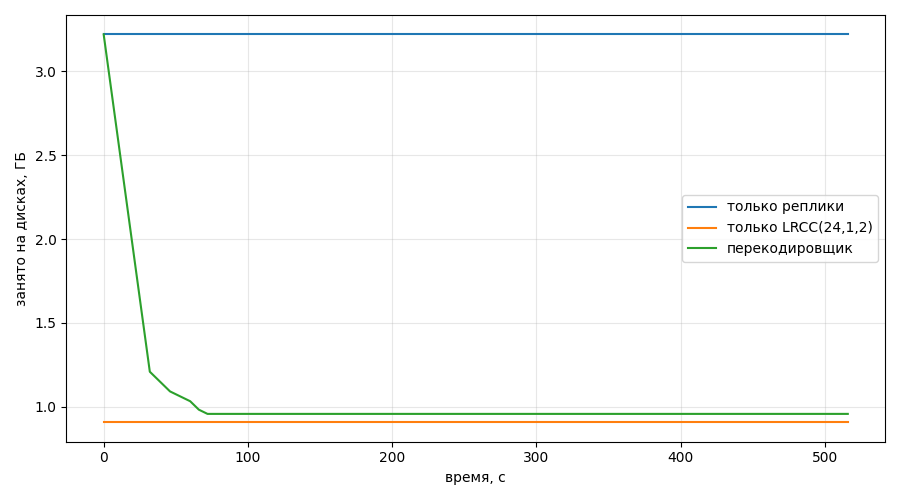
\includegraphics[width=0.92\textwidth]{images/experiments/cold_disk_used.png}
\caption{
\label{fig:cold-disk-used}
     Изменение занятого места после записи холодного объекта.}
\end{center}
\end{figure}

На рис.~\ref{fig:cold-disk-used} видно, что режим только с репликацией остаётся
на верхней границе по занимаемому месту, а режим только LRCC(24,1,2) задаёт
нижнюю границу. Перекодировщик начинает с того же состояния, что и репликация,
но затем постепенно переводит схемы в состояние с преобладанием проверочных
блоков и приближается к LRCC. Это показывает основную ожидаемую динамику: если
данные не читаются, реплики становятся избыточно дорогим способом хранения.
\FloatBarrier

\subsection{Длительная запись и фоновые переходы}

Следующий сценарий добавляет продолжительную запись новых объектов. Во время
записи перекодировщик не всегда успевает немедленно перевести все новые схемы в
LRCC, потому что фоновые переходы имеют задержку и ограничиваются числом
доступных локальных планировщиков.

\begin{figure}[!htbp]
\begin{center}
   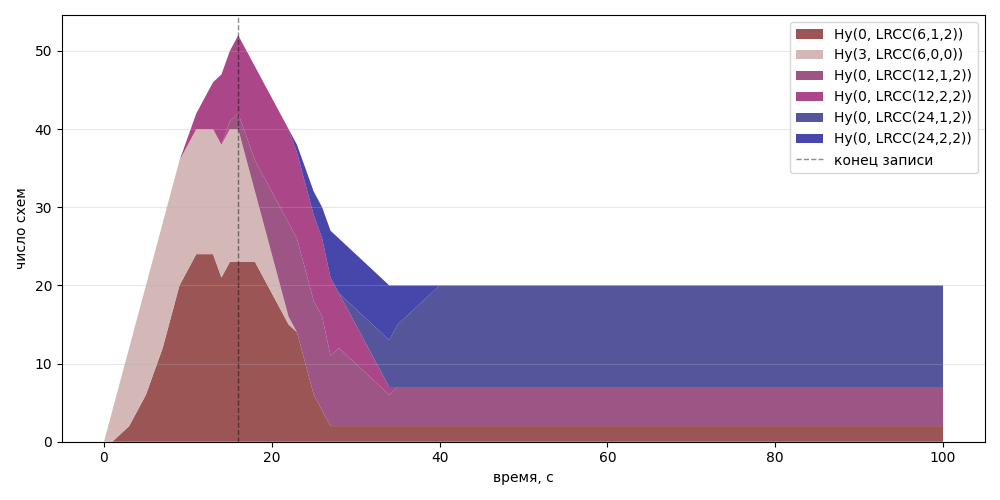
\includegraphics[width=0.92\textwidth]{images/experiments/continuous_scheme_distribution.png}
\caption{
\label{fig:continuous-scheme-distribution}
     Распределение точных сигнатур схем при продолжительной записи и
     последующем ожидании.}
\end{center}
\end{figure}

На рис.~\ref{fig:continuous-scheme-distribution} видно накопление схем с
преобладанием реплик во время активной записи. После окончания записи фоновые
переходы догоняют накопившуюся очередь, и почти все пользовательские блоки
переходят в широкие LRCC-состояния. Этот график полезен тем, что показывает не
только конечное состояние, но и инерционность системы: перекодирование является
фоновым процессом, а не мгновенной частью пути записи.
\FloatBarrier

\subsection{Неравномерная температура данных}

Равномерные случайные чтения часто размазывают температуру по объектам и не
создают ярко выраженных горячих или холодных областей. Поэтому отдельно
рассматривается нагрузка с распределением Ципфа
\cite{zipf1949human,breslau1999zipf}: логическое пространство объектов заранее
разбивается на куски, после чего вероятность чтения куска пропорциональна
обратной степени его ранга. Такой сценарий приближает модель к типичной
нагрузке систем хранения, где небольшая часть данных читается существенно чаще
остальных.

\begin{figure}[!htbp]
\begin{center}
   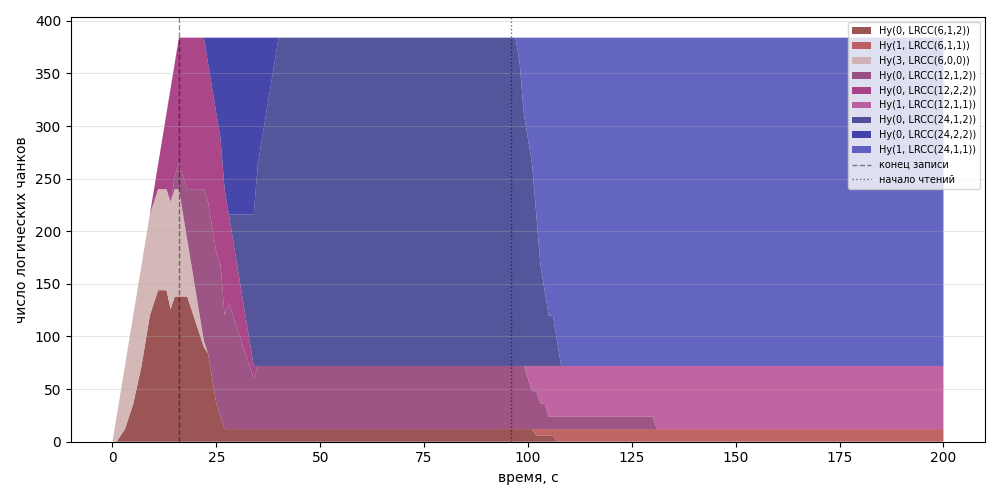
\includegraphics[width=0.92\textwidth]{images/experiments/logical_chunk_distribution.png}
\caption{
\label{fig:zipf-scheme-distribution}
     Распределение блоков данных по сигнатурам схем при чтениях по распределению Ципфа.}
\end{center}
\end{figure}

На рис.~\ref{fig:zipf-scheme-distribution} сначала при бездействии схемы
остывают, затем после начала чтения часть данных переходит в гибридные
состояния, так как для горячих областей выигрыш по чтению оказывается важнее
дополнительного расхода места. Это ключевой эксперимент для проверки
адаптивности: система реагирует не только на факт записи, но и на последующую
температуру отдельных схем.
\FloatBarrier

\subsection{Чтения при отказах}

Для оценки цены отказов моделируются сбои на случайных узлах: при
недоступности блока данных чтение восстанавливает его синхронно из локальных
или глобальных проверочных блоков, не меняя метаданные и не выполняя фоновое
восстановление. Отказ в экспериментах вносится как пометка узла недоступным.
В более интенсивном сценарии одновременно недоступны до трёх узлов с
LRCC-блоками данных, а набор отказавших узлов периодически меняется по кругу.

\begin{figure}[!htbp]
\begin{center}
   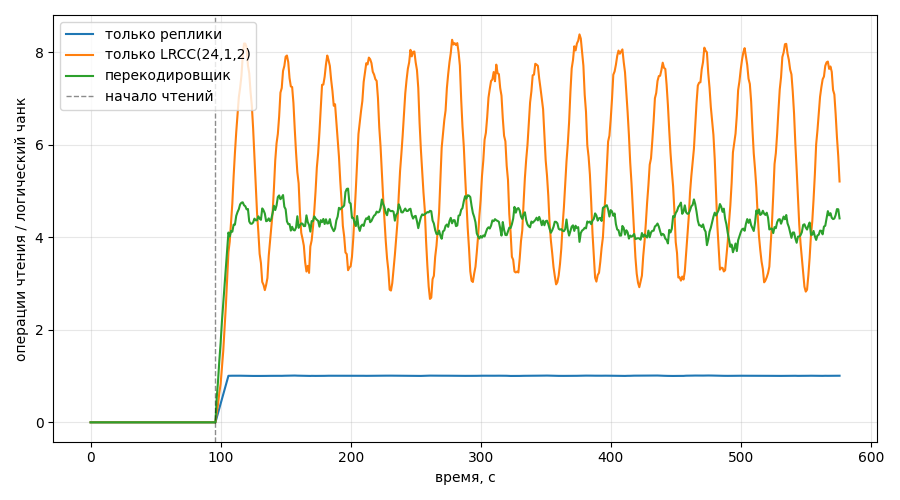
\includegraphics[width=0.92\textwidth]{images/experiments/avg_real_read_ops_smoothed.png}
\caption{
\label{fig:stress-read-ops}
     Сглаженное число операций чтения на логический блок при случайных чтениях
     и интенсивных отказах.}
\end{center}
\end{figure}

На рис.~\ref{fig:stress-read-ops} режим только LRCC(24,1,2) показывает пики,
потому что читает блоки данных и избыточности для восстановления. Схема
широкая, поэтому статистически очень вероятны отказы в схеме, располагающейся
почти по всем узлам. Репликация почти не чувствительна к такому сценарию, пока
среди доменов отказа, хранящих прямые размещения нужного блока, доступен хотя
бы один. Перекодировщик занимает промежуточное положение: часть данных хранится
компактно, но горячие или рискованные схемы могут оставаться в более удобном
для чтения состоянии.
\FloatBarrier

\subsection{Смешанный жизненный цикл}

Наиболее близкий к целевому поведению сценарий объединяет несколько фаз:
продолжительную запись, простой, чтения по распределению Ципфа и затем
равномерные случайные чтения. Он нужен, чтобы проверить, что система не
оптимизируется под один искусственный момент времени, а меняет состояние при
смене характера нагрузки.

\begin{figure}[!htbp]
\begin{center}
   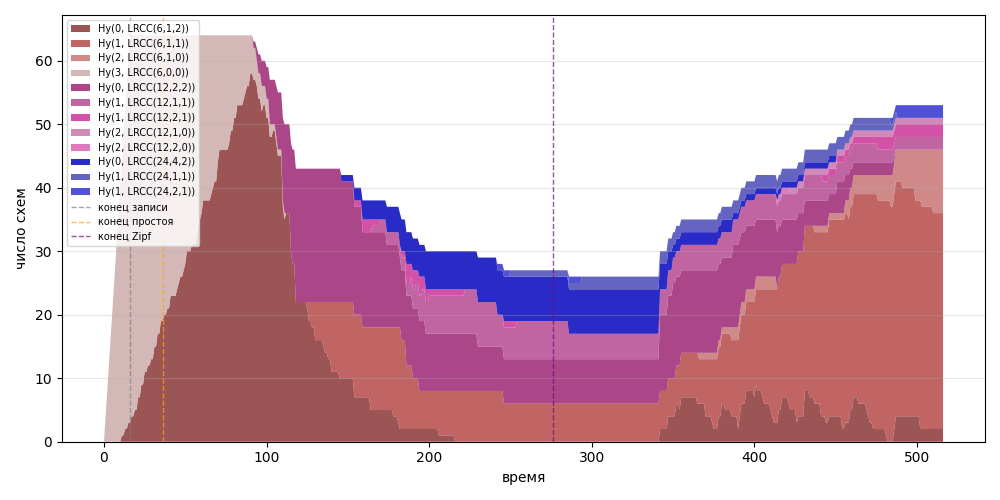
\includegraphics[width=0.92\textwidth]{images/experiments/scheme_distribution.png}
\caption{
\label{fig:mixed-scheme-distribution}
     Изменение распределения схем в смешанном сценарии:
     запись, простой, чтения по распределению Ципфа и случайные чтения.}
\end{center}
\end{figure}

На рис.~\ref{fig:mixed-scheme-distribution} после фазы записи и простоя схемы
уходят в широкие LRCC, что соответствует холодному хранению. Затем во время
чтений часть схем возвращается в гибридные состояния с преобладанием реплик
или разделяется на более узкие схемы. После смены распределения чтений меняется
и баланс типов схем. Более того, меняется и количество схем --- это связано с
их объединениями и разделениями. Этот график наиболее полно демонстрирует идею
конвертируемых кодов в данной работе
\cite{maturana2022convertible,kong2024lrcconvertible}: код не выбирается один
раз навсегда, а становится управляемым состоянием жизненного цикла данных.
\FloatBarrier

\subsection{Выводы по экспериментам}

Проведённые эксперименты подтверждают ожидаемое поведение предложенного
подхода. Во-первых, для холодных данных перекодировщик приближается к
эффективности LRCC по занимаемому месту. Во-вторых, при неравномерной
температуре он сохраняет часть схем в более дорогих по месту, но дешёвых по
чтению состояниях. В-третьих, при отказах чистый LRCC выигрывает по месту, но
платит ростом числа чтений при восстановлении и задержки; адаптивный режим
позволяет частично сгладить этот компромисс.

Таким образом, основная ценность предложенной схемы состоит не в том, чтобы
заменить репликацию или кодирование стираний одним фиксированным кодом, а в
том, чтобы сделать выбор схемы динамическим и локальным для разных частей
данных.

\FloatBarrier
\pagebreak

\specialsection{Заключение}

Выполненная работа показала, что схема отказоустойчивого хранения может
рассматриваться не как фиксированный выбор между репликацией и кодированием
стираний, а как автоматически управляемое состояние данных. Для данных с
дозаписью такой подход позволяет локально менять форму избыточности в фоне:
сохранять дешёвое чтение для более активных участков и компактнее хранить
менее активные данные. Поставленная во введении цель настоящей работы
достигнута: предложенный подход соответствует требованиям отказоустойчивости и
позволяет автоматически менять форму избыточности между состояниями с
преобладанием реплик и состояниями с преобладанием проверочных блоков в
зависимости от активности данных, занятого места, ожидаемой стоимости чтения и
стоимости фонового перехода между схемами.

В ходе работы были получены следующие результаты:
\begin{itemize}
    \item проанализированы существующие подходы к отказоустойчивому хранению:
    репликация, коды стираний, локально восстанавливаемые и конвертируемые
    коды, температурные политики и системы с изменением схемы хранения;
    \item сформулирована модель гибридного хранения и температуры данных как
    численной метрики текущей интенсивности чтений;
    \item определены допустимые переходы между схемами, включая обмен
    реплик на проверочные блоки, обратные переходы, изменение числа
    локальных групп, объединение и разделение совместимых схем;
    \item разработана модель оценки полезности перехода, учитывающая занятое
    место, ожидаемую стоимость чтения и стоимость фонового перекодирования;
    \item спроектирована архитектура адаптивного выбора переходов и разработана
    экспериментальная система \nolinkurl{https://github.com/v131v/hybrid_distributed_storage} с фоновым перекодировщиком, локальными
    планировщиками и глобальным планировщиком;
    \item проведена экспериментальная оценка поведения системы при охлаждении
    данных, неравномерной нагрузке чтения и отказах узлов.
\end{itemize}

Все поставленные задачи были выполнены. Экспериментальные данные показали, что
предложенный подход в рассмотренных сценариях позволяет одновременно более эффективно
использовать дисковое пространство по сравнению с исключительно репликацией и снижать
задержку операций чтения по сравнению с исключительно кодированием стираний.
Также показана способность адаптироваться к разным типам нагрузки на примере
случайных чтений и чтений, распределённых по закону Ципфа. При этом сохраняется
отказоустойчивость: в рассмотренных сценариях отказов запросы чтения
продолжали обрабатываться по пути чтения с восстановлением.

Ограничения работы связаны с выбранной постановкой и уровнем реализации.
Рассматривалась append-нагрузка: запись новых объектов и дозапись существующих
без изменения уже закрытых полос данных. Фоновое восстановление физически
утраченных блоков было отделено от задачи адаптивного перекодирования. Кроме
того, планировщик итеративно выбирает следующий лучший переход, что не
гарантирует глобального оптимума конфигурации. Предложенный подход также не
предназначен для мгновенной реакции на резкие изменения нагрузки.

Дальнейшее развитие работы может включать добавление механизма фонового
восстановления, проверку политики планирования на реальных распределениях
температуры данных, а также исследование масштабирования распределения
ответственности локальных планировщиков для крупных объектов и больших
кластеров. Тем не менее уже полученные результаты подтверждают основную
гипотезу: адаптивная смена схемы избыточности может быть полезным механизмом
управления способом хранения данных в отказоустойчивом хранилище.

\pagebreak


% 4) Список литературы
\printbibliography[heading=bibintoc,title={Список литературы}]

% 5) Приложения (пример)
% \appendix
% \section{Приложение A. Дополнительные материалы}

Здесь можно размещать объёмные таблицы, листинги, дополнительные графики и т.п.

\pagebreak



\end{document}
